% This is my HW 8 solution set.

\documentclass[12pt, leqno]{article}
\usepackage{amsfonts, amsmath, amssymb}
\usepackage{amsbsy}
\usepackage{fancyhdr}
\usepackage{hyperref}
\usepackage{graphicx}
\newcounter{qcounter}
%\usepackage[landscape]{geometry}% http://ctan.org/pkg/geometry
%\usepackage{array}% http://ctan.org/pkg/array
\usepackage[lofdepth,lotdepth]{subfig}
\usepackage[maxfloats=40]{morefloats}
\usepackage{float}
\usepackage{}
\usepackage[english]{babel}
\usepackage{tabularx}
\usepackage{scalerel}
\providecommand{\abs}[1]{\lvert#1\rvert} % absolute value
\providecommand{\normd}{\mathcal{N}} % normal distribution
\providecommand{\norm}[1]{\lVert#1\rVert} % norm
\usepackage{mathtools}
\DeclarePairedDelimiter\ceil{\lceil}{\rceil}
\DeclarePairedDelimiter\floor{\lfloor}{\rfloor}
\newcommand{\macheps}{\epsilon_{\mbox{\scriptsize mach}}}
\usepackage[ampersand]{easylist}
\makeatletter
\newcommand{\distas}[1]{\mathbin{\overset{#1}{\kern\z@\sim}}}%
\newsavebox{\mybox}\newsavebox{\mysim}
\newcommand{\distras}[1]{%
  \savebox{\mybox}{\hbox{\kern3pt$\scriptstyle#1$\kern3pt}}%
  \savebox{\mysim}{\hbox{$\sim$}}%
  \mathbin{\overset{#1}{\kern\z@\resizebox{\wd\mybox}{\ht\mysim}{$\sim$}}}%
}
\makeatother
%\usepackage{pdflscape}


\begin{document}
\pagestyle{fancy}
\lhead{Syed Rahman}
\rhead{STA6866}

\begin{center}
{\large {\bf Project}} \\
\end{center}

\paragraph{} We are interested in finding the hospital with the best
mortaility rate, which is equivalent to finding the hospital with the
lowest $E(\lambda_i)$. We run a Gibbs-Sampler for the following model:
\begin{align}
Z_i & \sim Poisson(\lambda_i e_i), \notag \\
\lambda_i & \sim Gamma(\alpha, \beta), \notag \\
\alpha & \sim Exp(a_0), \qquad{} a_0 = \log(2)/z_0, \qquad{} z_0 = 0.53, \notag \\
\beta & \sim Gamma(b_0, b_1),  \qquad{} b_0 = 1, \qquad{} b_1 = 0.65, \notag 
\end{align}
and estimate the mortality rate of hospital $i$, $E(\lambda_i)$, using 
\[
\widehat{E(\lambda_i)} = \frac{1}{n} \sum_{j=1}^n \lambda_i^{(j)} = \bar{\lambda}_i,
\]
where $n$ is the number of observations collected in our sample and $\lambda_i^{(j)}$
denotes the $j$th observation for $\lambda_i$.

Note that under this model, the value of the log of the posterior
denisty of $(\pmb{\lambda},{\alpha},{\beta})$ at
$(\pmb{\hat{\lambda}},\hat{\alpha},\hat{\beta}) =
(\hat{\lambda}_1,... \hat{\lambda}_{94},\hat{\alpha},\hat{\beta})$ can
be calculated in the following manner:
\begin{align}
f_{(\pmb{\lambda},{\alpha},{\beta})|\pmb{Z}} (\pmb{\hat{\lambda}},\hat{\alpha},\hat{\beta}) &=
c \prod_{i=1}^{94} f_{Z_i|\hat{\lambda}_i}(Z_i)
f_{\lambda_i|(\hat{\alpha},\hat{\beta})}(\hat{\lambda}_i)
f_{{\alpha}}(\hat{\alpha}) f_{{\beta}}(\hat{\beta})\notag \\
\implies \log f_{(\pmb{\lambda},{\alpha},{\beta})|\pmb{Z}} (\pmb{\hat{\lambda}},\hat{\alpha},\hat{\beta}) 
&= \log c + 
\sum_{i=1}^{94} \big(\log f_{Z_i|\hat{\lambda}_i}(Z_i) + 
\log f_{\lambda_i|(\hat{\alpha},\hat{\beta})}(\hat{\lambda}_i)
\notag \\ 
&\qquad + \log f_{{\alpha}}(\hat{\alpha}) + \log
f_{{\beta}}(\hat{\beta}) \big)
\notag 
\end{align}
where $c$ is the normalzing constant, which we will ignore when
plotting the posterior density.

We initially run a Gibbs-Sampler on the model using $JAGs$ with a thin of $1$, a burn-in of $10000$ and
$n=50000$ with initial values of $\lambda_i^{(0)} = 1 \forall i$. Figure \ref{cumsumt1}
indicates that the negative log posterior converges slowly
to a value around 900, but Figures \ref{logpostt1} and \ref{logpost2t1} indicates
that it exhibits a clear
sinusoidal pattern. This
indicates that the chains generated by this algorithm are most
likely getting stuck in regions from which it takes a significant
amount of time to escape; in other words, they are $mixing \: slowly$.  The trace plots for $\alpha$ and $\beta$ in Figure \ref{alphaacft1}
and \ref{betaacft1} also seem problematic for the same reason. As expected, the
autocorrelation plots for $\alpha$ and $\beta$ in
Figure \ref{alphaacft1} and \ref{betaacft1}
reveal extremely high
correlation. These plots indicate that a thin of $100$ may work better. 

We run another Gibbs-Sampler on the same model again using $JAGs$ with a thin of 100, a burn-in of $10000$ and
$n=50000$ this time. Figures \ref{logpostt100}, \ref{logpost2t100} and
\ref{cumsumt100} shows that the negative log posterior for this chain
varies evenly around some value between 850 and 900 without getting stuck in any region for too
long. These look much better than when we used a thin of 1. Also, as
is evident in
Figure \ref{alphaacft100} and \ref{betaacft100}, the
autocorrelation plots for $\alpha$ and $\beta$ indicate that the thin
of $100$ works well. The trace plots for $\alpha$ and $\beta$ in Figure \ref{alphaacft100}
and \ref{betaacft100} also seem much better. 

The estimated means and
their standard errors, calculated employing the naive method, time series methods (TS) and
batch means (BM), using a thin of 1 and a thin of 100 are
reported in Table \ref{mean1} and Table \ref{mean100}, respectively. In calculating the standard errors using
the batch means method we used a batch size of
$\floor{n/ \sqrt{n}}$. As expected, the general trend is that 
variance estimates are smaller when using a thin of 100. With a thin
of 1 we also get significantly
different values for the standard errors using the different methods,
whereas the naive, TS and BM estimates are similar when using a thin of 100. This suggests
that the covariance term is almost $0$ for the sample collected using a thin of 100, which implies that it is $closer$
to an $iid$ sample. 

The ``best" mortality rates are for
hospitals $63$ and $85$ and the ``worst" mortality rates are for
hospitals $9$
and $68$. These are presented in Table \ref{bw} along with $95\%$ CI's,
which were calculated using the TS standard errors from the sample
collected with a thin of 100. Trace
plots and autocorrelation plots for these $\lambda_i$ are presented in Figures \ref{tracet1},
\ref{acft1}, \ref{tracet100} and \ref{acft100}. Interestingly enough,
the $\lambda_i$ corresponding to 
these are the hospitals that exhibited the most problematic autocorrelation
plots when using a thin of 1. It is also clear from Figure \ref{acft100} that autocorrelation amongst
the $\lambda_i$ is close of negligible using a thin of 100. Finally we tried
multiple starting points using a thin of 100 by setting the
initial values of $\lambda_i^{(0)} = 10 \forall i$, $\lambda_i^{(0)} = 100
\forall i$ and $\lambda_i^{(0)}$ as a random sample from the uniform
distribution on [1,100]
$\forall i$, which still gave us the same results in terms of
parameter and error
estimates and diagnostic plots. 

\begin{table}[ht]
\centering
\scalebox{0.8}{
\begin{tabular}{|r|r|r|}
  \hline
\hline
Best Hospitals:  &  
 Mortality Rates& $95\%$ CI  \\
\hline
85&0.368 & (0.366236,0.369764)\\
63&0.468 & (0.465648,0.470352)\\
\hline
Worst Hospitals:  &  
Mortality Rates& $95\%$ CI  \\
\hline
9&1.512 &  (1.506512,1.517488)\\
68&1.642  & ( 1.637688,1.646312)\\
\hline
\hline
\end{tabular}
}
\caption{Best and Worst Hospitals based on mortality rates using a thin of 100} 
\label{bw}
\end{table}

\clearpage

%\begin{landscape}

\begin{figure}
\centering
\subfloat[]
  {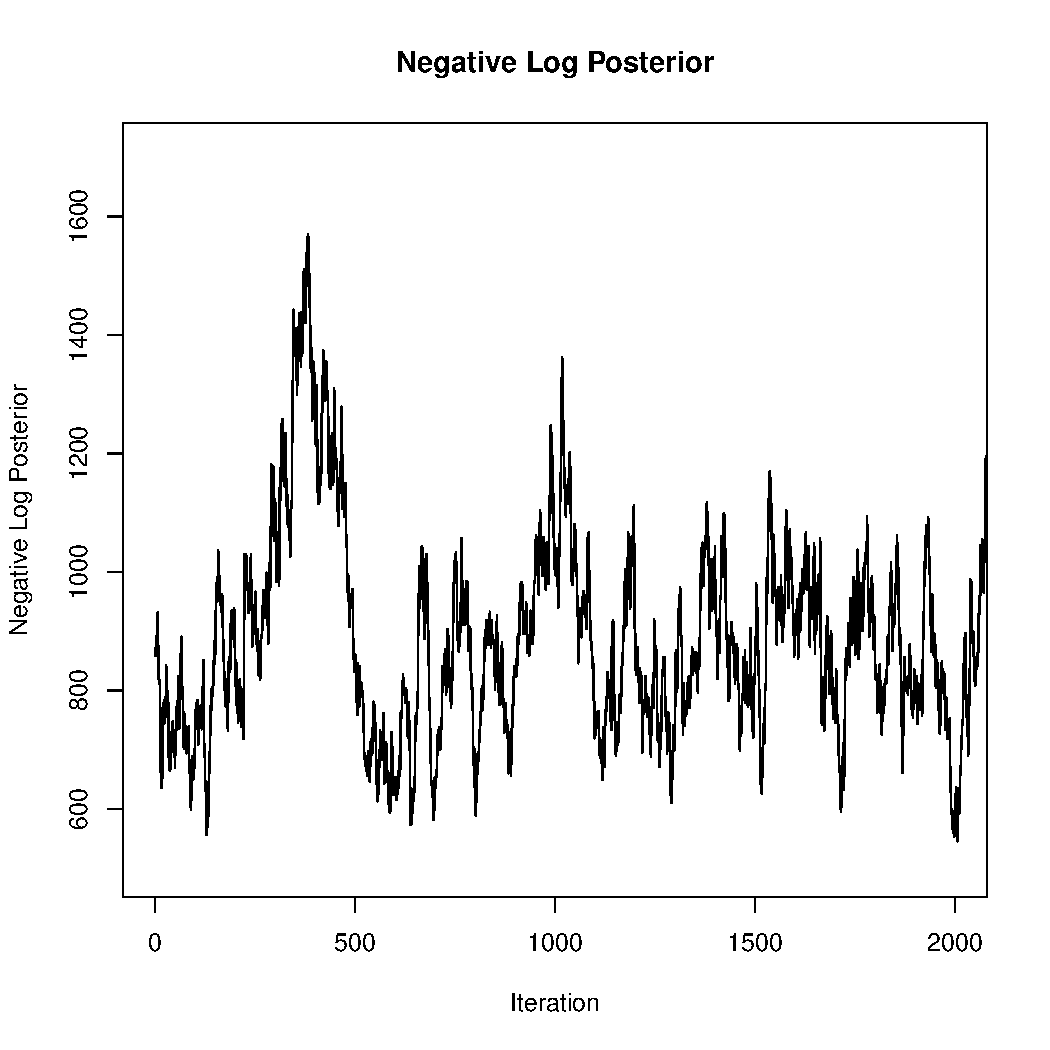
\includegraphics[scale=0.38]{logpostt1.pdf}
\label{logpostt1}}
\subfloat[]
  {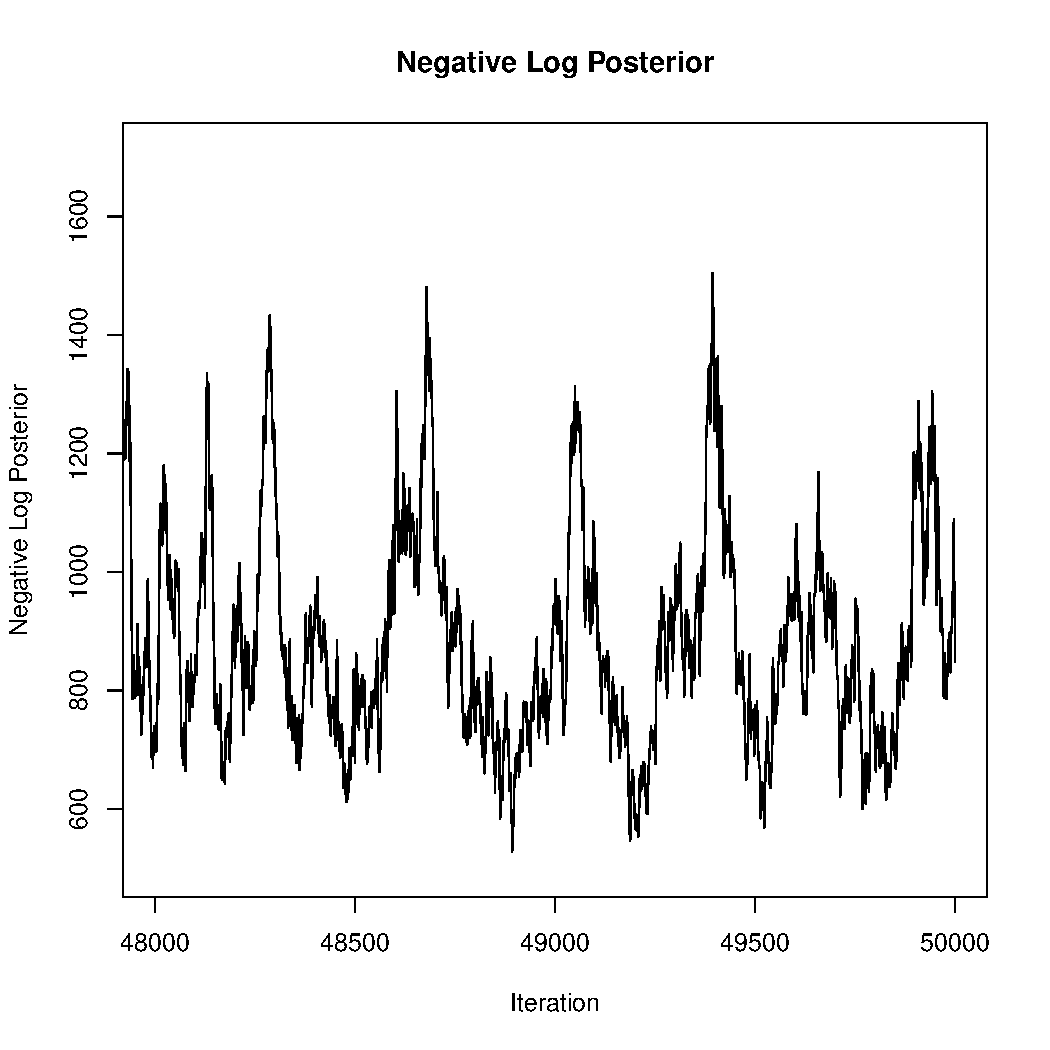
\includegraphics[scale=0.38]{logpost2t1.pdf}
\label{logpost2t1}}
\centering
\qquad
\centering
\subfloat[]
  {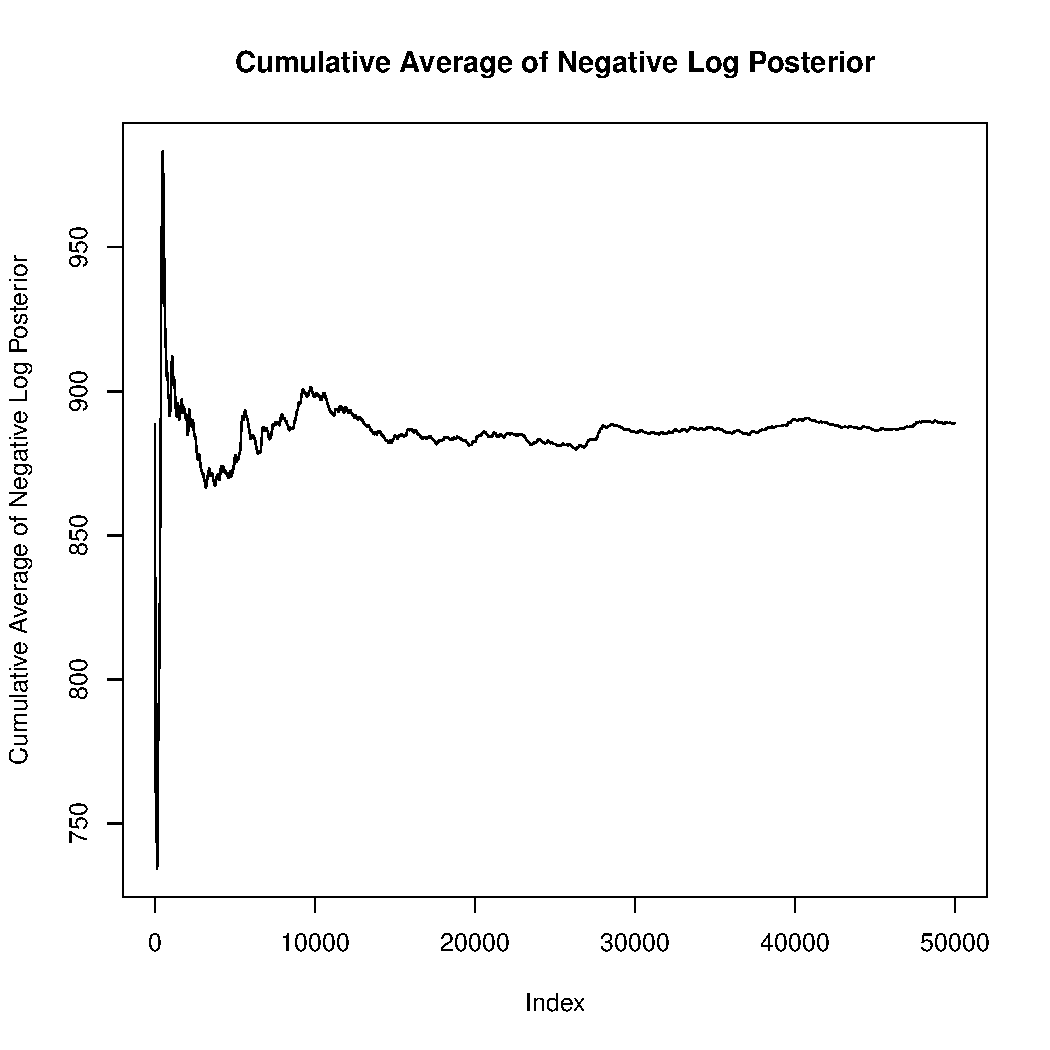
\includegraphics[scale=0.45]{cumsumt1.pdf}
\label{cumsumt1}}
\caption{Negative Log Posterior with a thin of 1}
\end{figure}

\begin{figure}
\centering
\subfloat[]
  {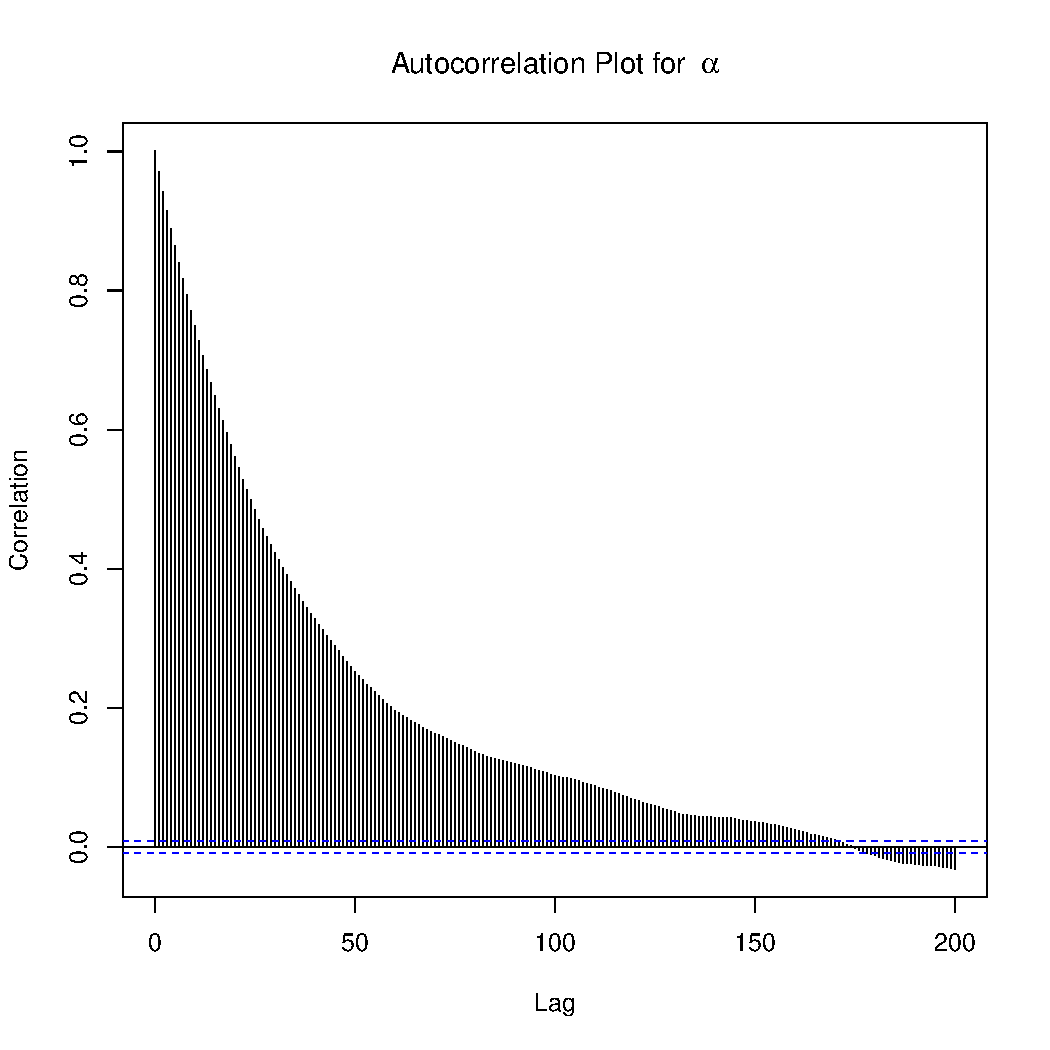
\includegraphics[scale=0.45]{alphaacft1.pdf}
\label{alphaacft1}}
\centering
\qquad
\centering
\subfloat[]
  {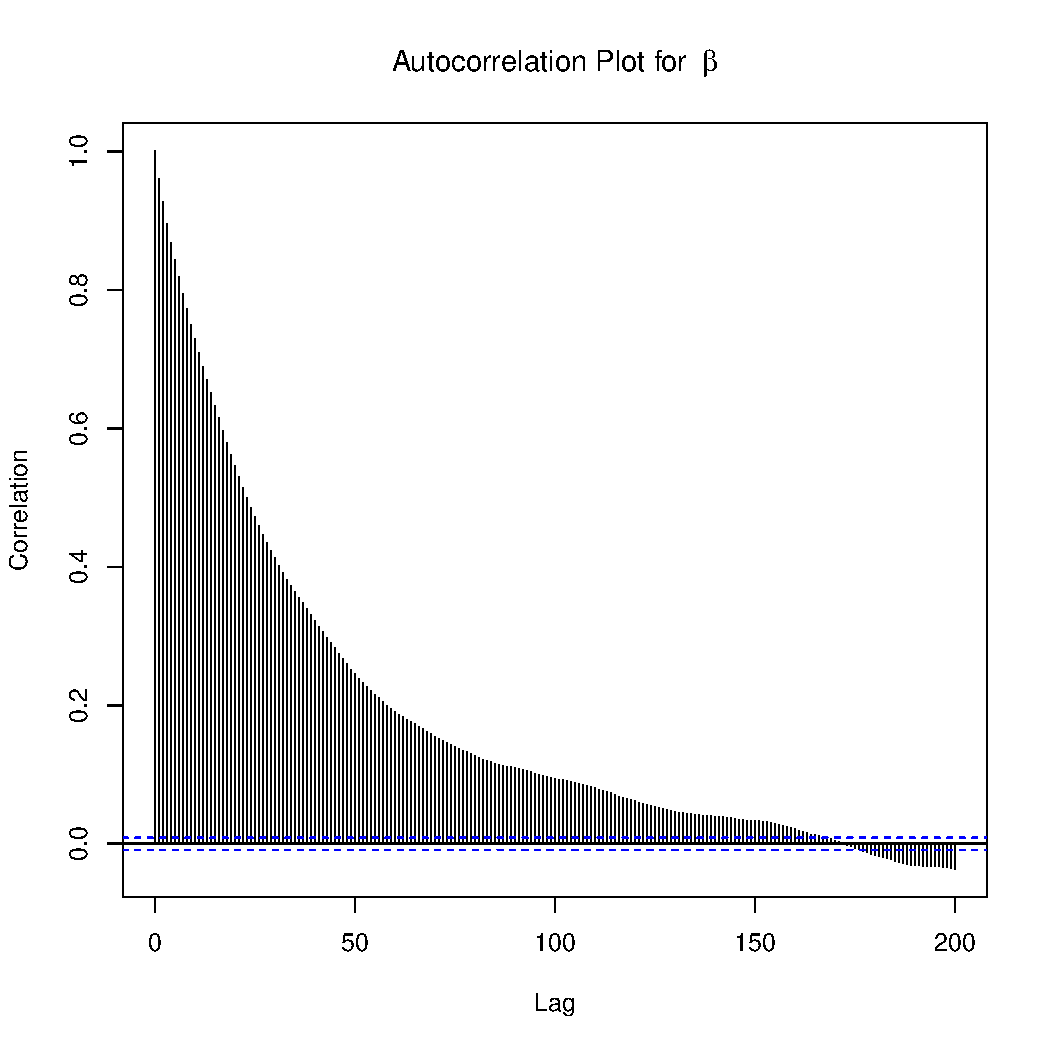
\includegraphics[scale=0.45]{betaacft1.pdf}
\label{betaacft1}}
\caption{Auto-Correlation plot for $\alpha$ in Figure \ref{alphaacft1}
  and $\beta$ in Figure \ref{betaacft1} with a thin of 1}
\end{figure}


\begin{figure}
\centering
\subfloat[]
  {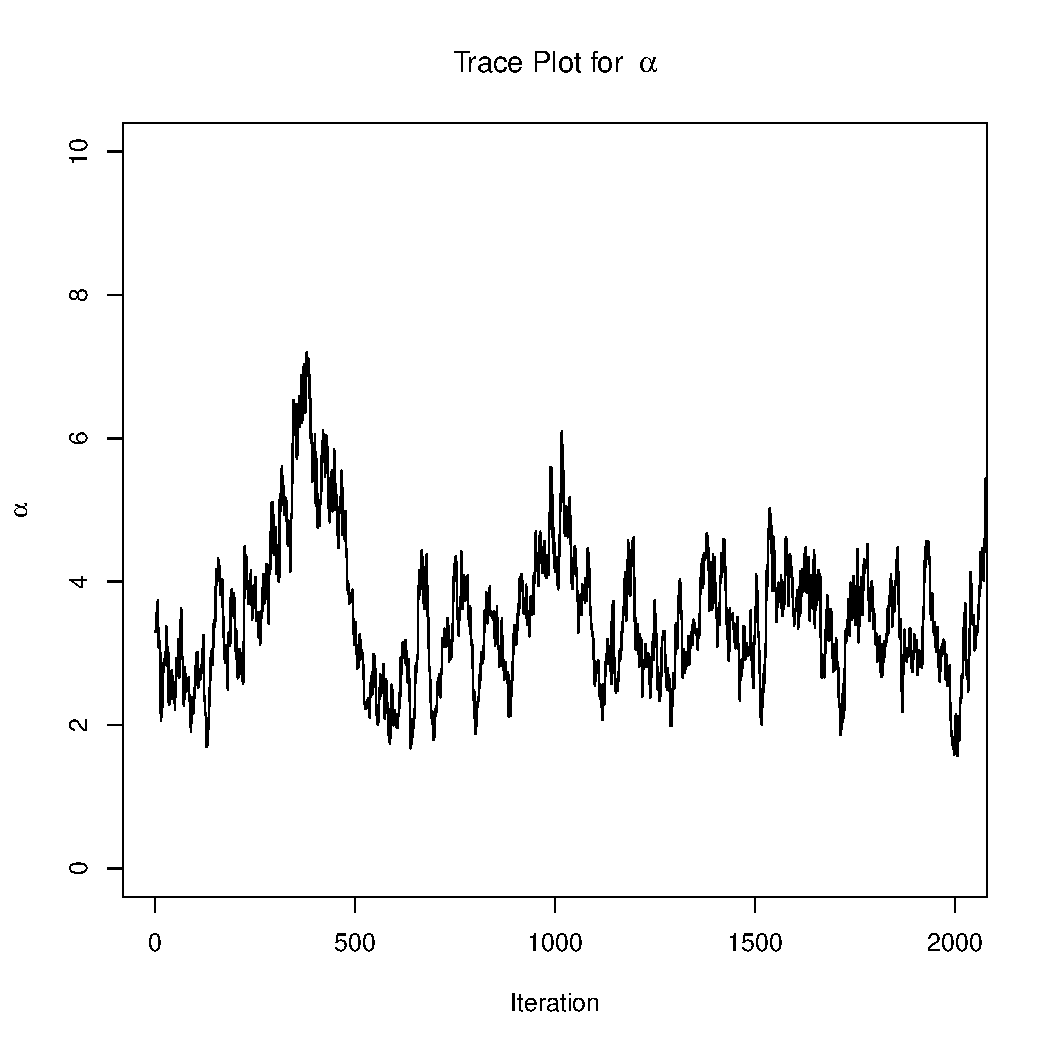
\includegraphics[scale=0.45]{alphat1.pdf}
\label{alphat1}}
\centering
\qquad
\centering
\subfloat[]
  {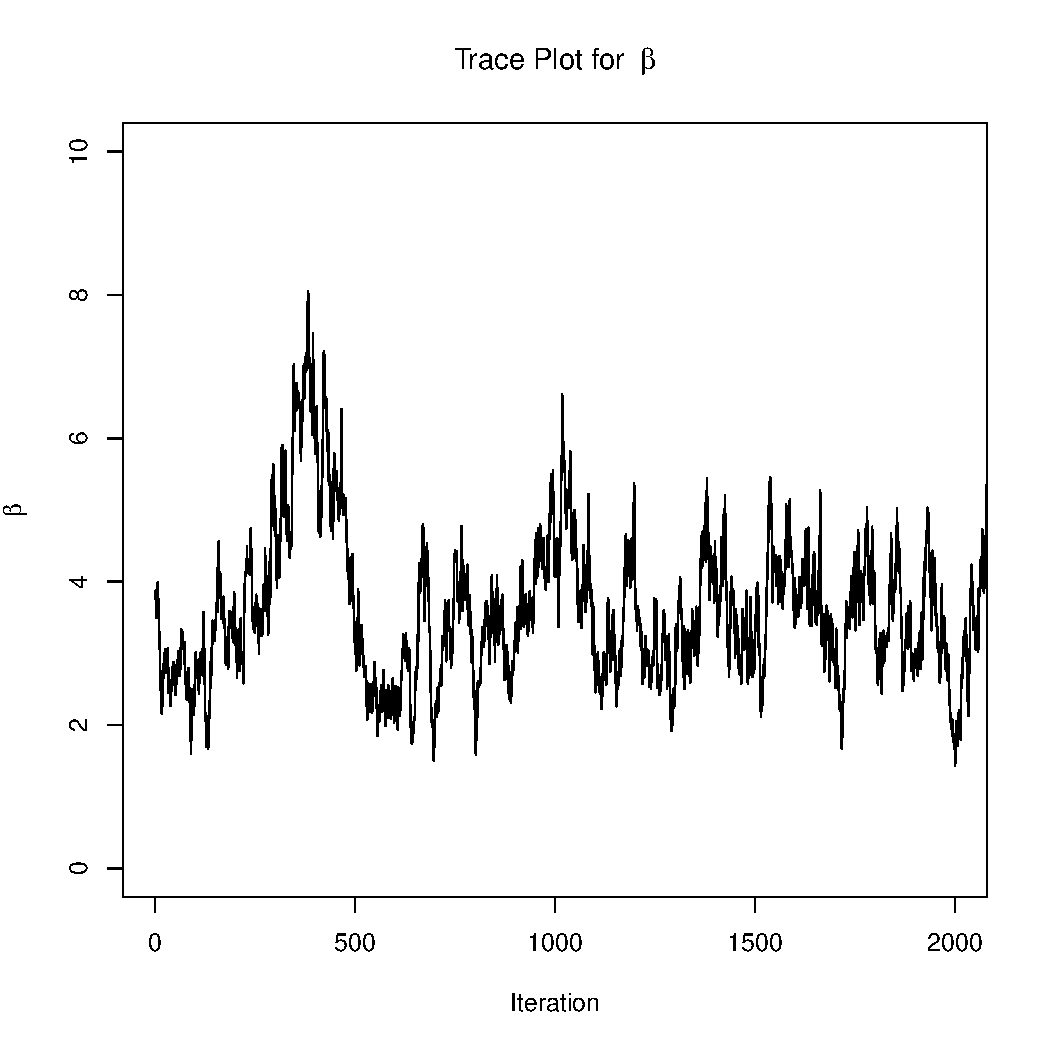
\includegraphics[scale=0.45]{betat1.pdf}
\label{betat1}}
\caption{Trace plot for $\alpha$ in Figure \ref{alphat1}  and $\beta$ in Figure \ref{betat1}  with a thin of 1}
\end{figure}

\begin{figure}
\centering
\subfloat[]
  {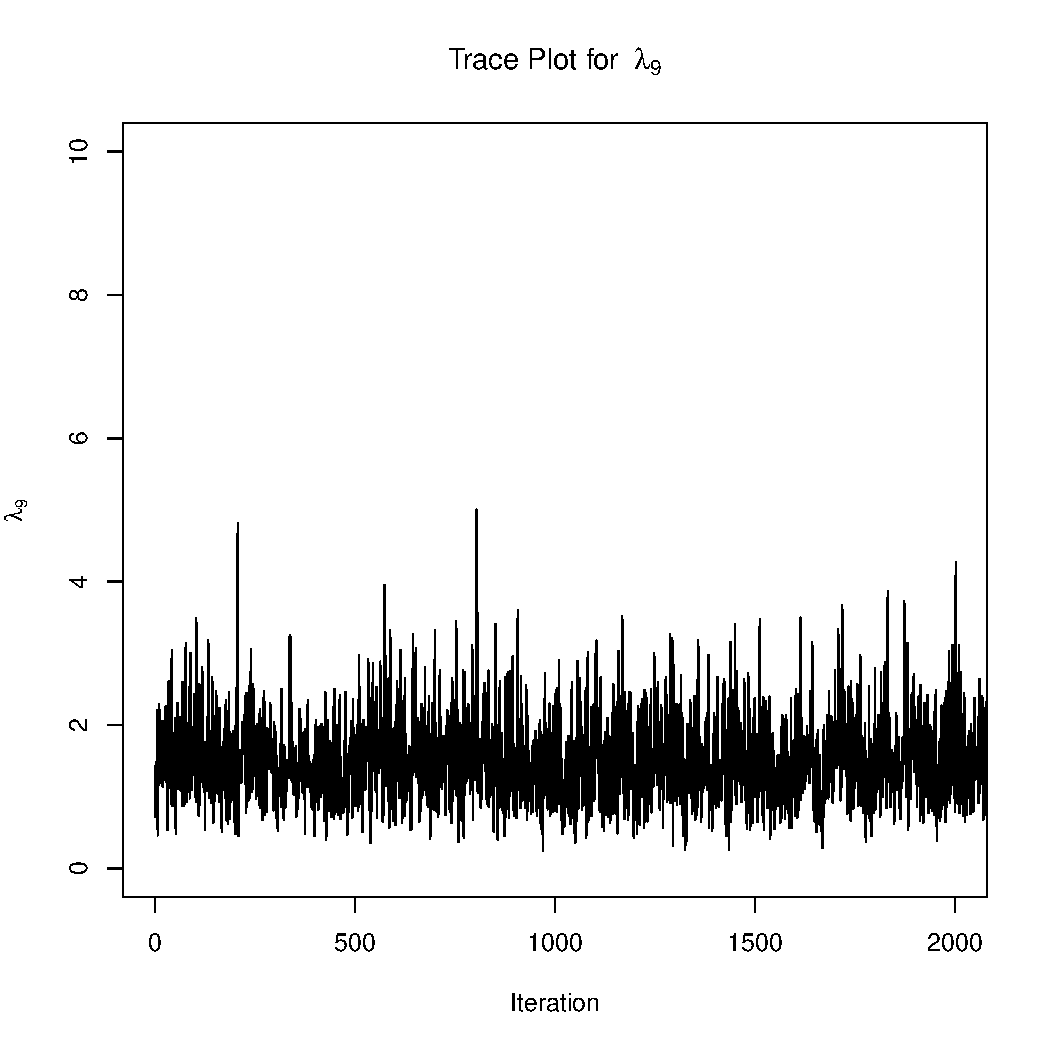
\includegraphics[scale=0.38]{tracelmd9t1.pdf}
\label{tracelmd9t1}}
\subfloat[]
  {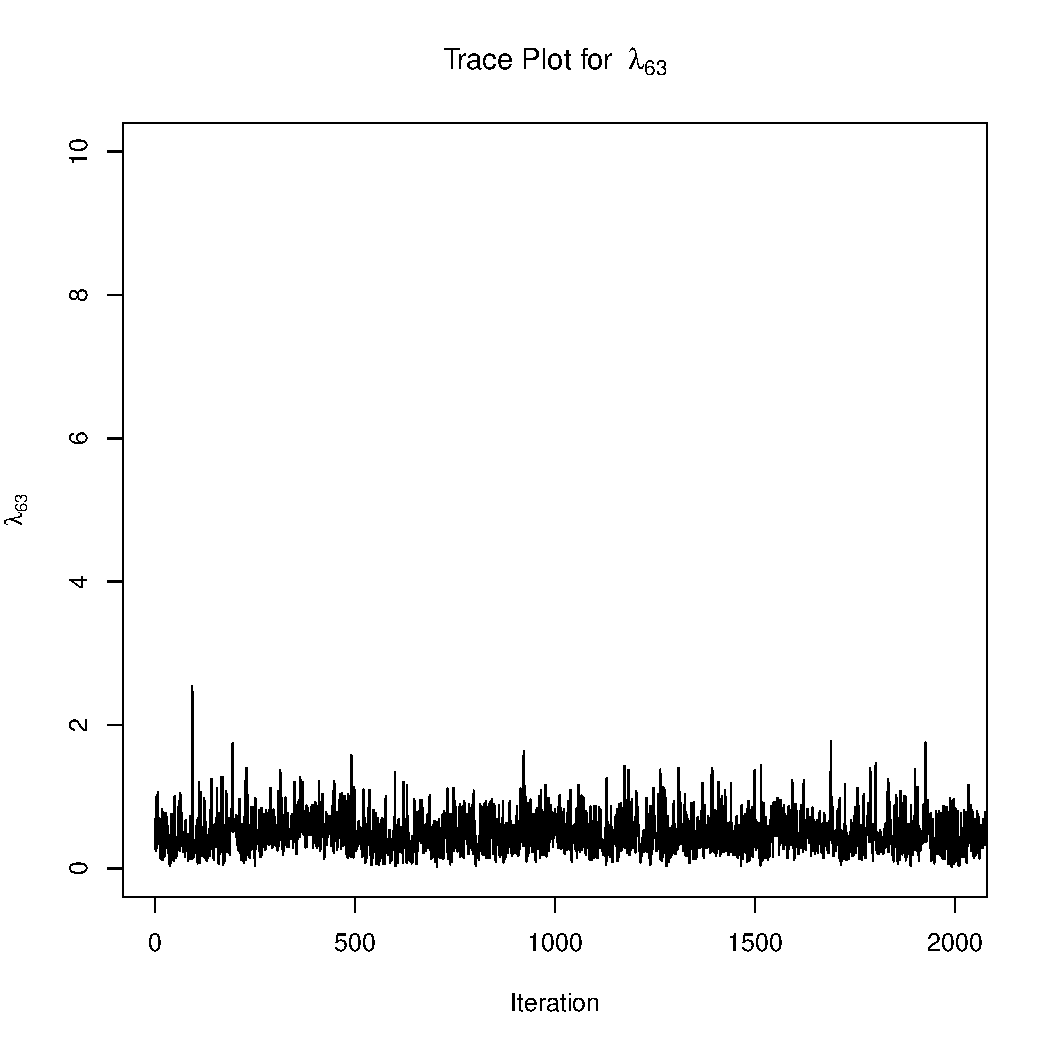
\includegraphics[scale=0.38]{tracelmd63t1.pdf}
\label{tracelmd63t1}}
\centering
\qquad
\centering
\subfloat[]
  {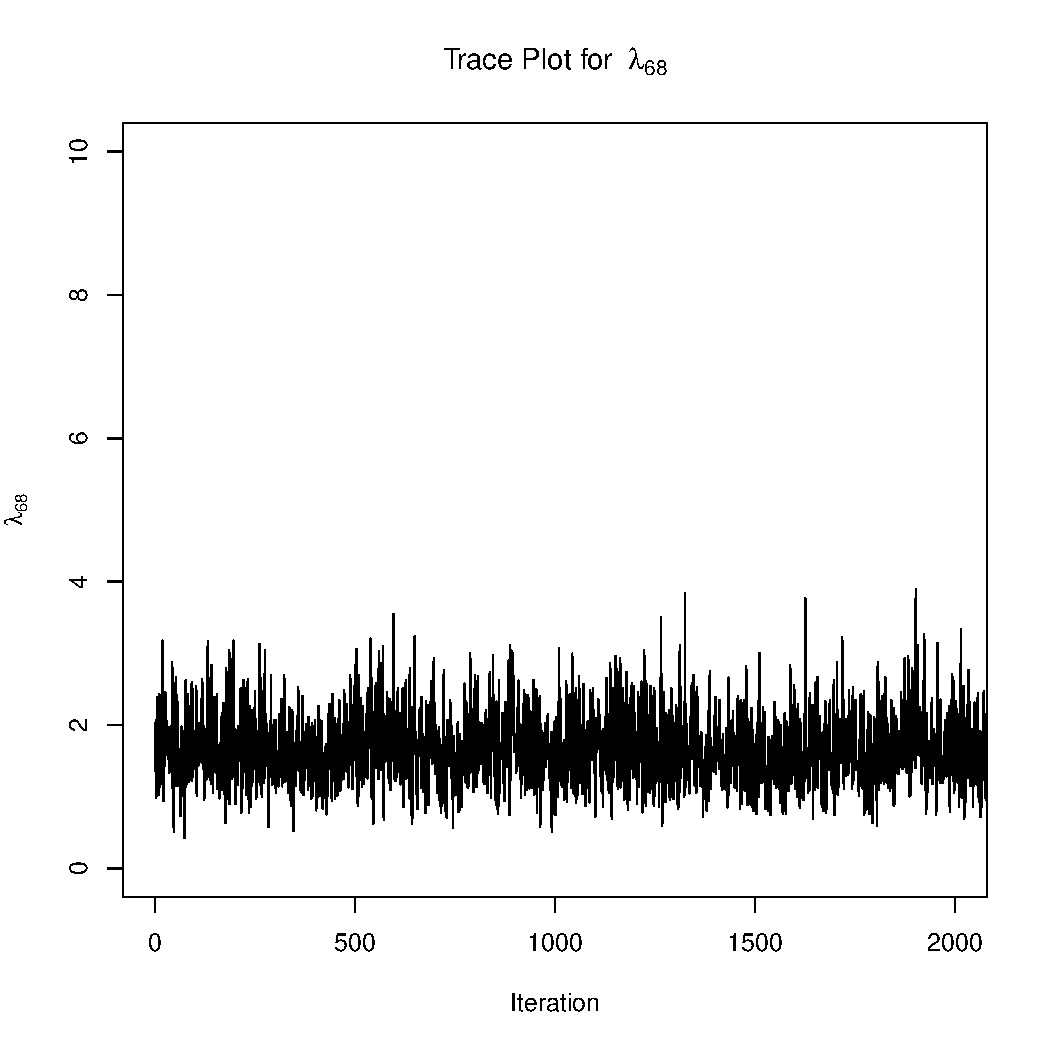
\includegraphics[scale=0.38]{tracelmd68t1.pdf}
\label{tracelmd68t1}}
\subfloat[]
  {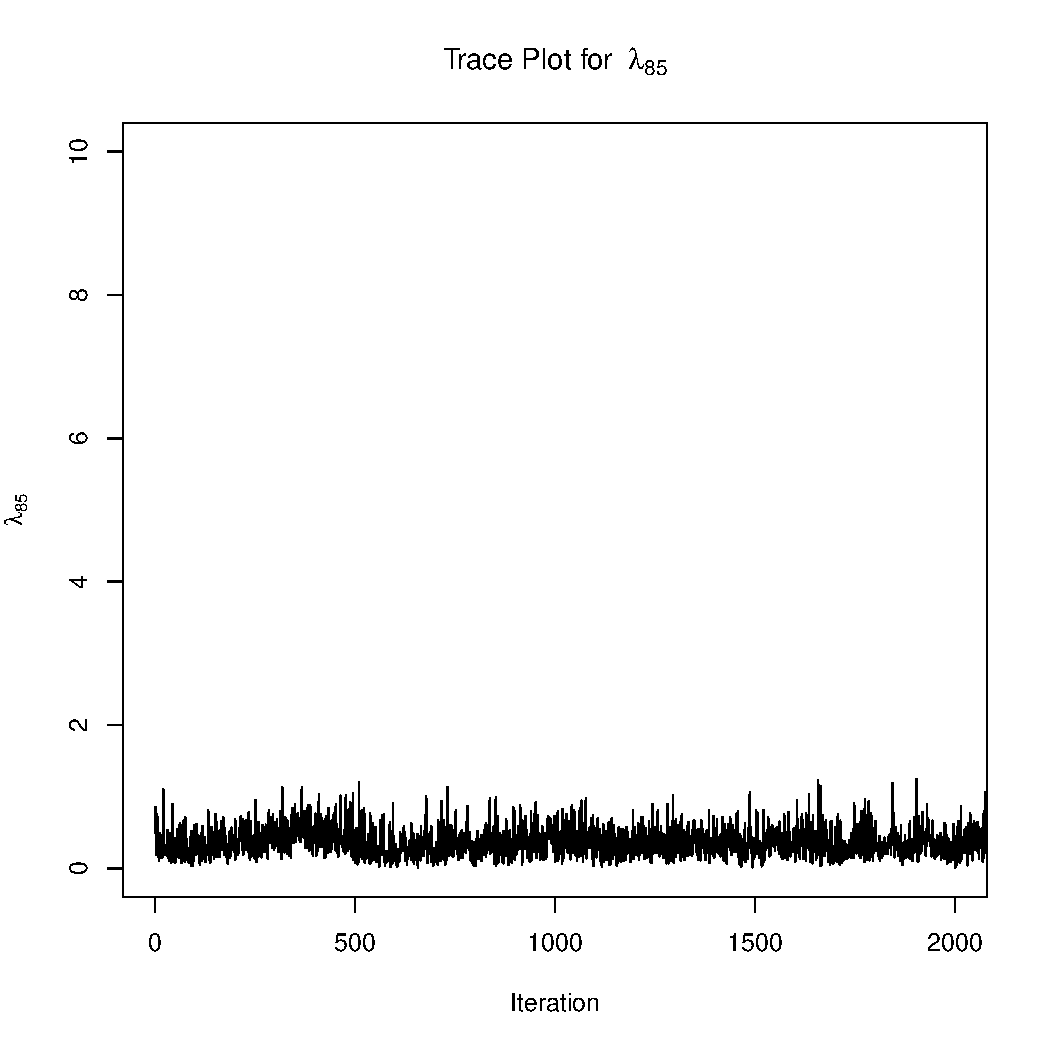
\includegraphics[scale=0.38]{tracelmd85t1.pdf}
\label{tracelmd85t1}}
\caption{Trace Plots for $\lambda_i$ using a thin of 1}
\label{tracet1}
\end{figure}

\begin{figure}
\centering
\subfloat[]
  {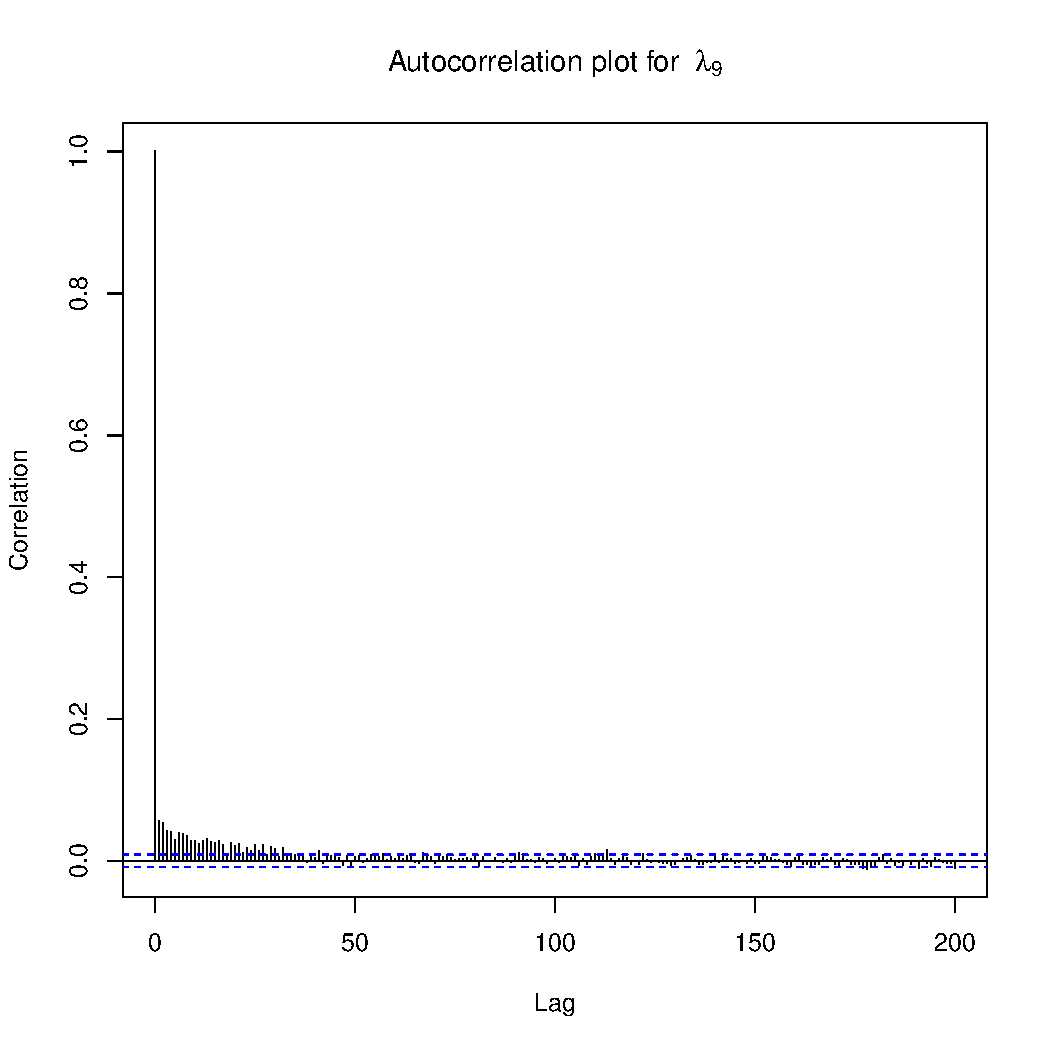
\includegraphics[scale=0.38]{acf9t1.pdf}
\label{acf9t1}}
\subfloat[]
  {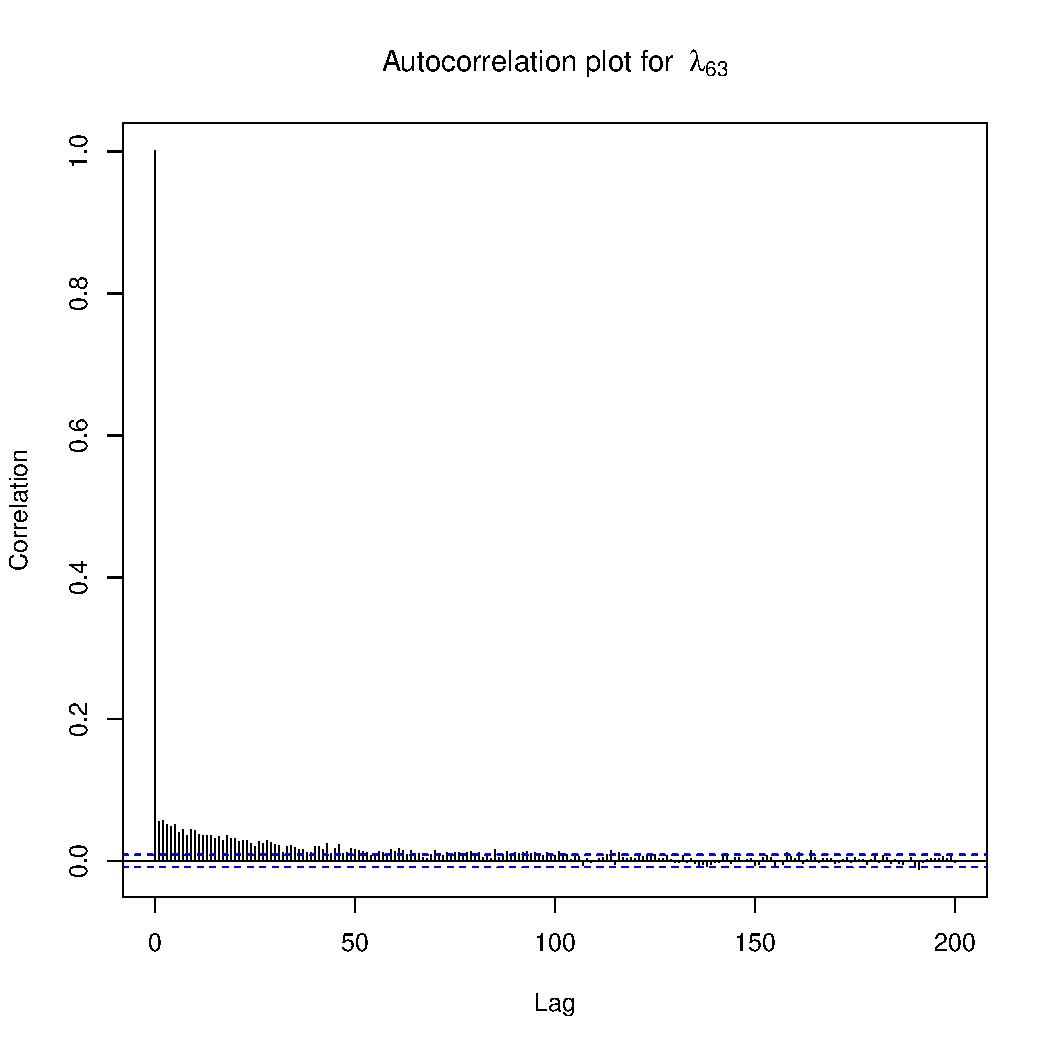
\includegraphics[scale=0.38]{acf63t1.pdf}
\label{acf63t1}}
\centering
\qquad
\centering
\subfloat[]
  {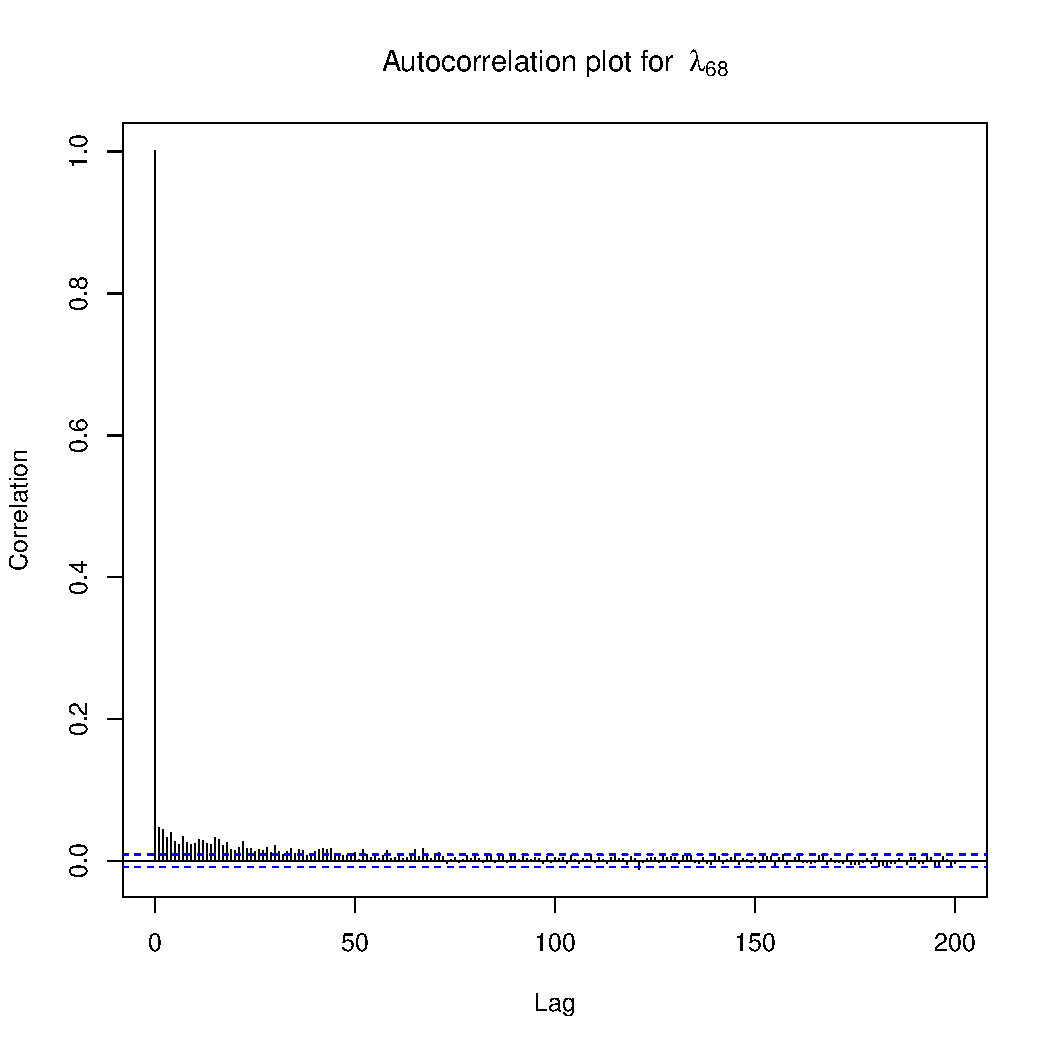
\includegraphics[scale=0.38]{acf68t1.pdf}
\label{acf68t1}}
\subfloat[]
  {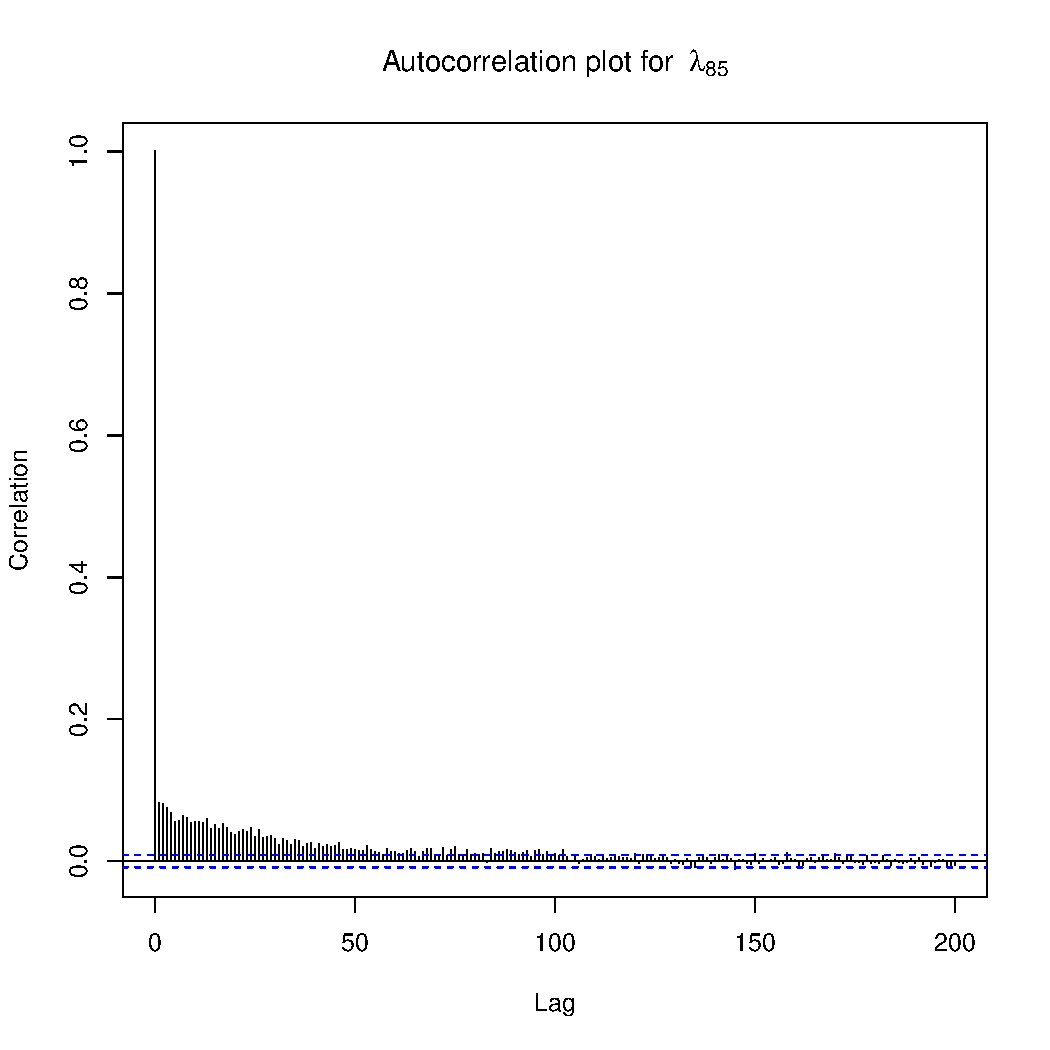
\includegraphics[scale=0.38]{acf85t1.pdf}
\label{acf85t1}}
\caption{Autocorrelation Plots for $\lambda_i$ using a thin of 1}
\label{acft1}
\end{figure}


\begin{figure}
\centering
\subfloat[]
  {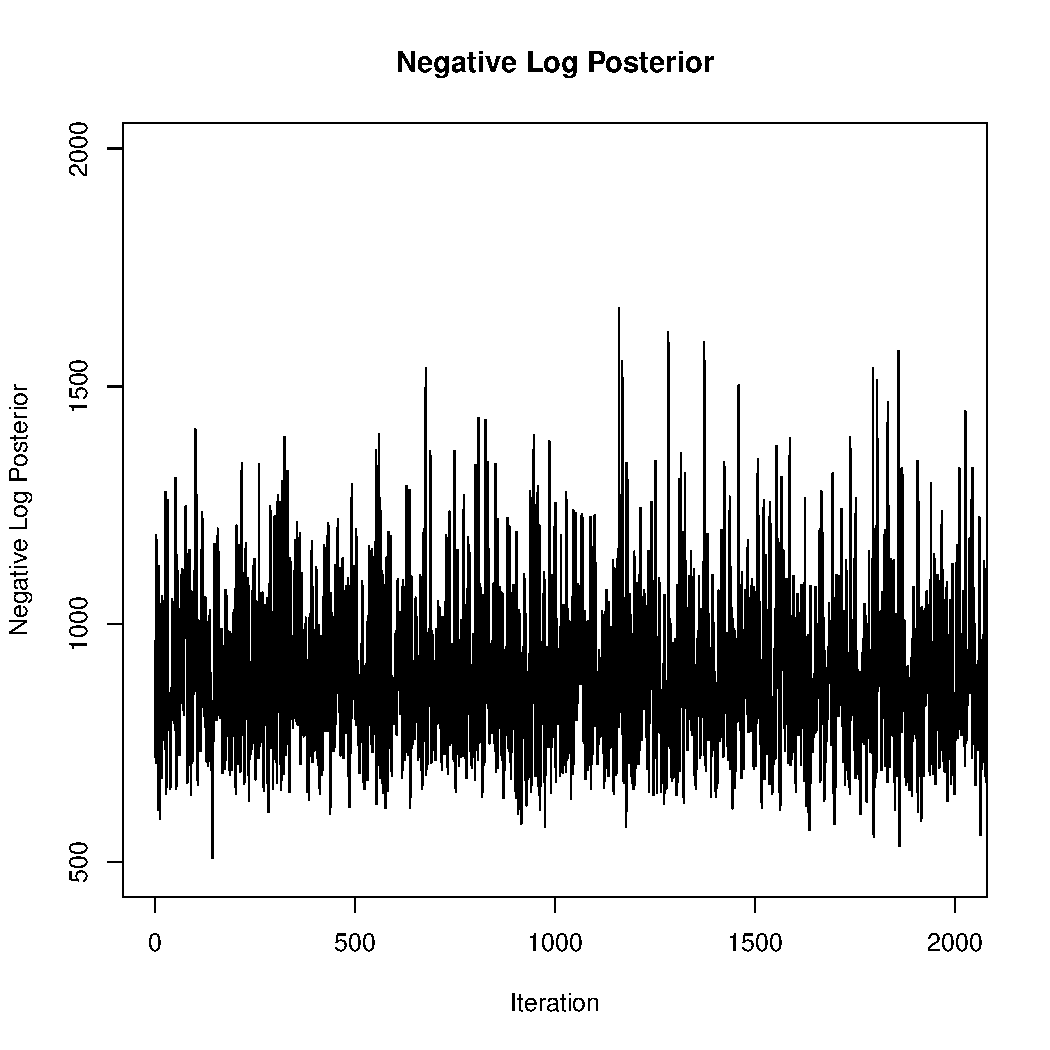
\includegraphics[scale=0.38]{logpostt100.pdf}
\label{logpostt100}}
\subfloat[]
  {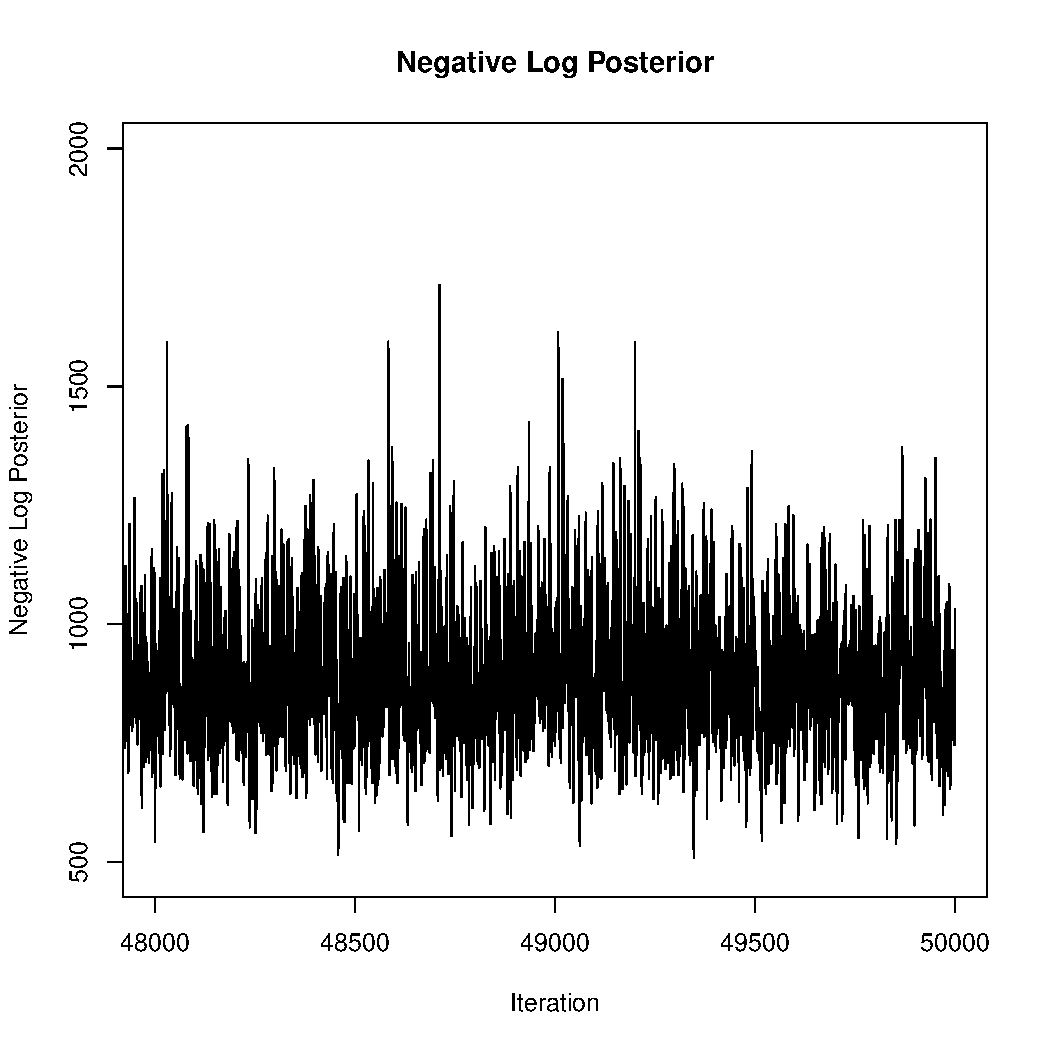
\includegraphics[scale=0.38]{logpost2t100.pdf}
\label{logpost2t100}}
\qquad
\centering
\subfloat[]
  {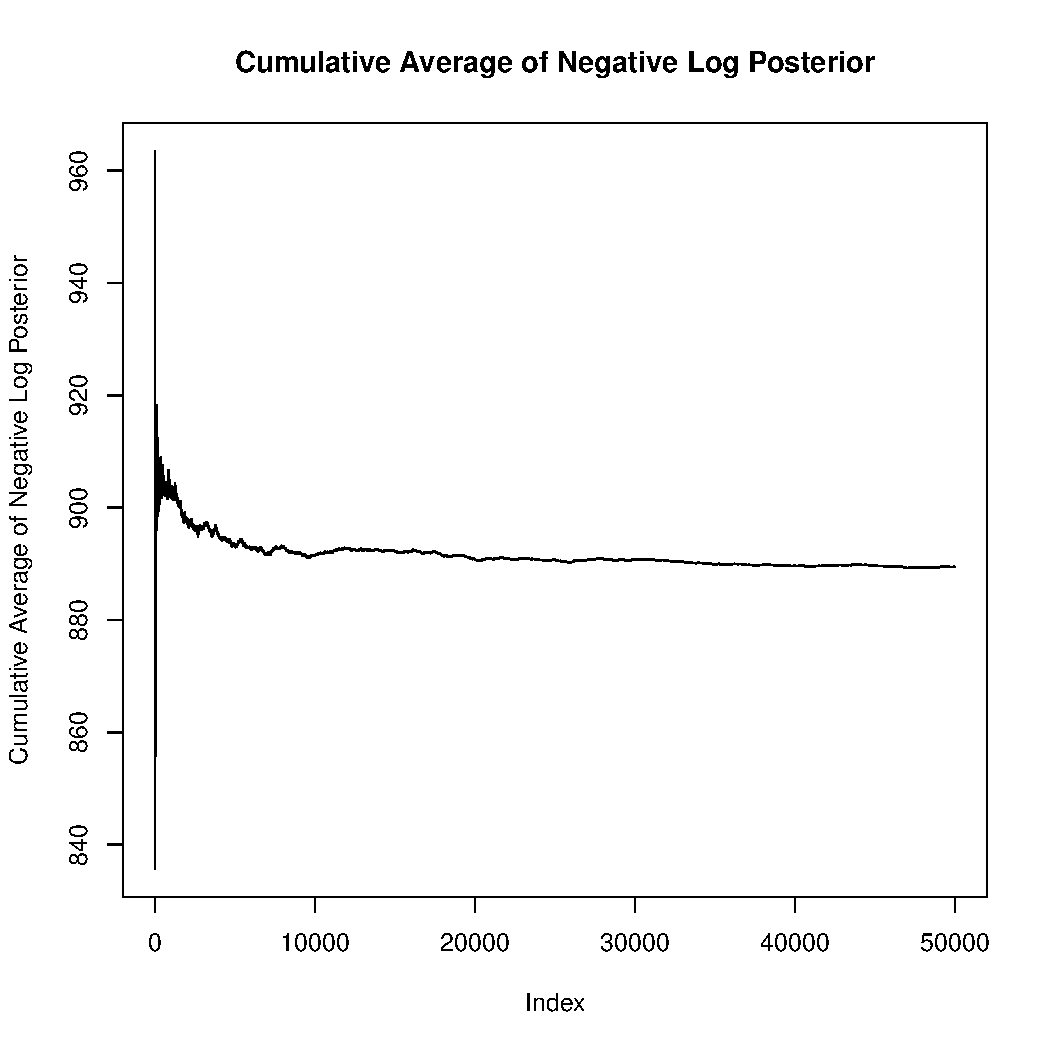
\includegraphics[scale=0.45]{cumsumt100.pdf}
\label{cumsumt100}}
\caption{Negative Log Posterior with a thin of 100}
\end{figure}



\begin{figure}
\centering
\subfloat[]
  {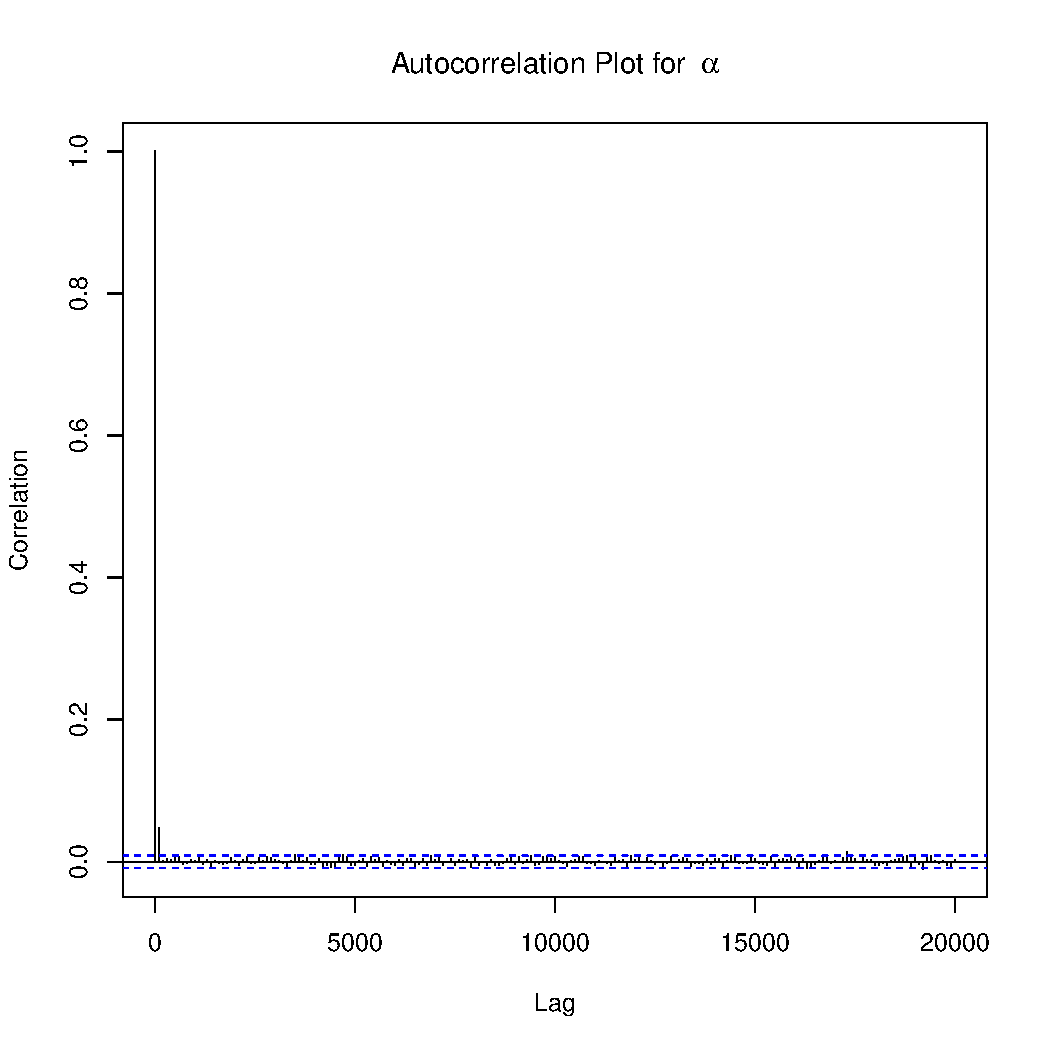
\includegraphics[scale=0.45]{alphaacft100.pdf}
\label{alphaacft100}}
\centering
\qquad
\centering
\subfloat[]
  {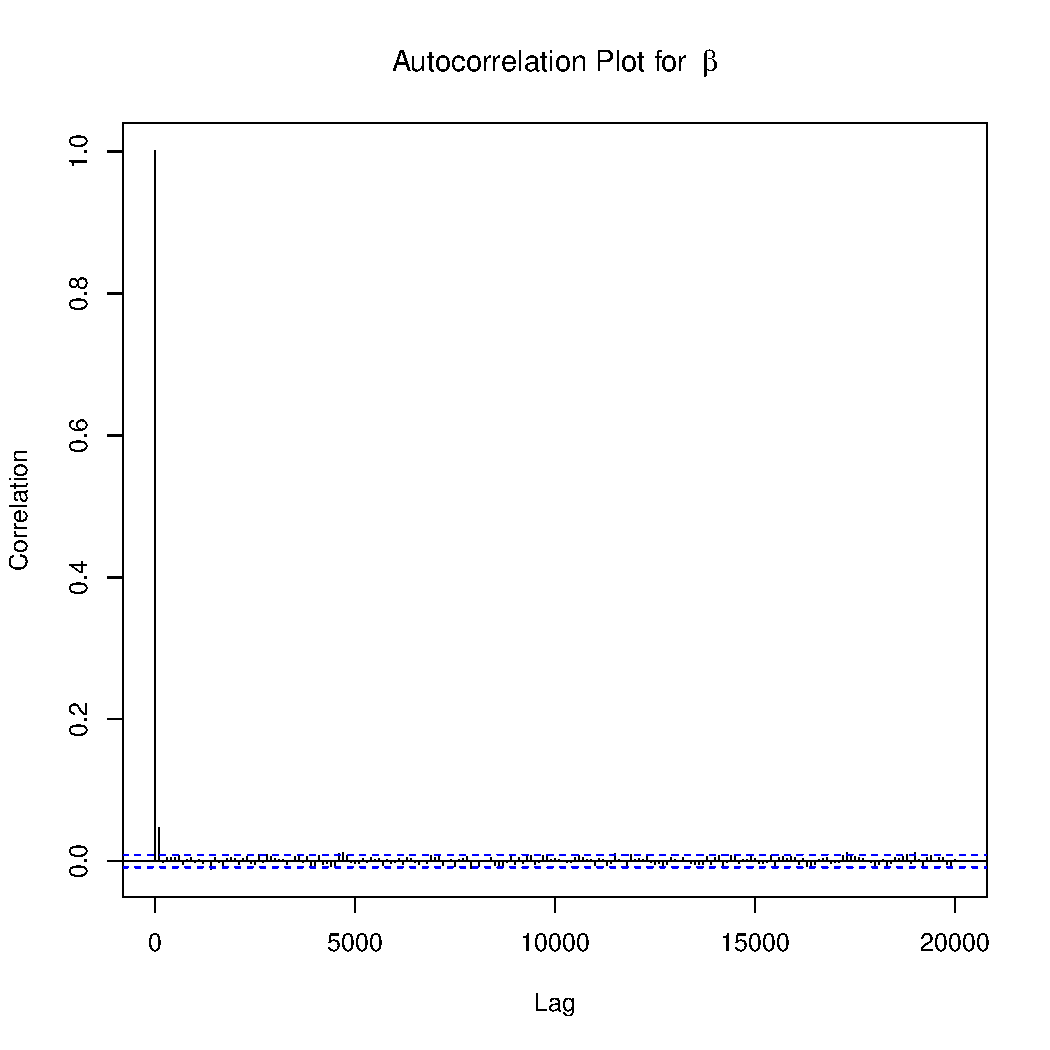
\includegraphics[scale=0.45]{betaacft100.pdf}
\label{betaacft100}}
\caption{Auto-Correlation plot for $\alpha$ in Figure \ref{alphaacft100} and $\beta$ in Figure \ref{betaacft100} with a thin of 100}
\end{figure}


\begin{figure}
\centering
\subfloat[]
  {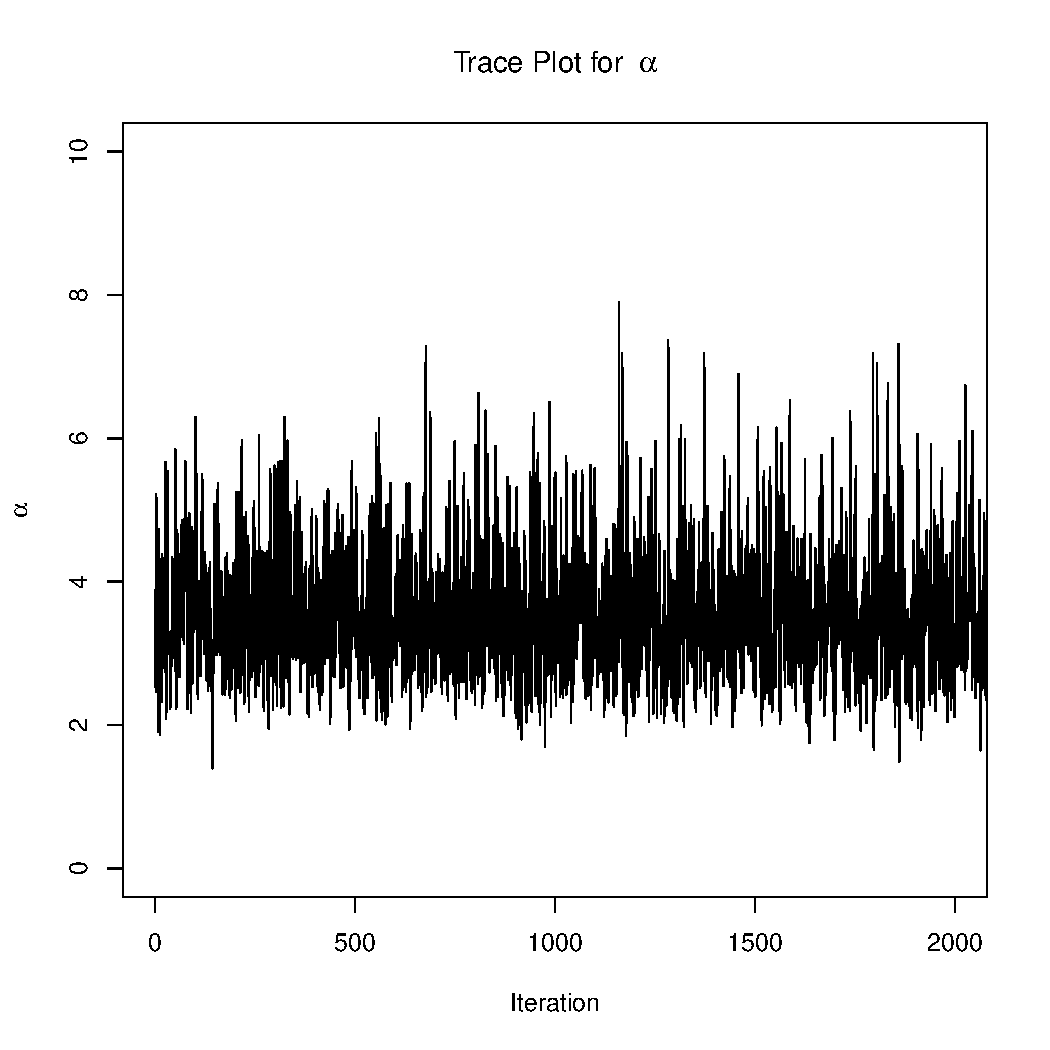
\includegraphics[scale=0.45]{alphat100.pdf}
\label{alphat100}}
\centering
\qquad
\centering
\subfloat[]
  {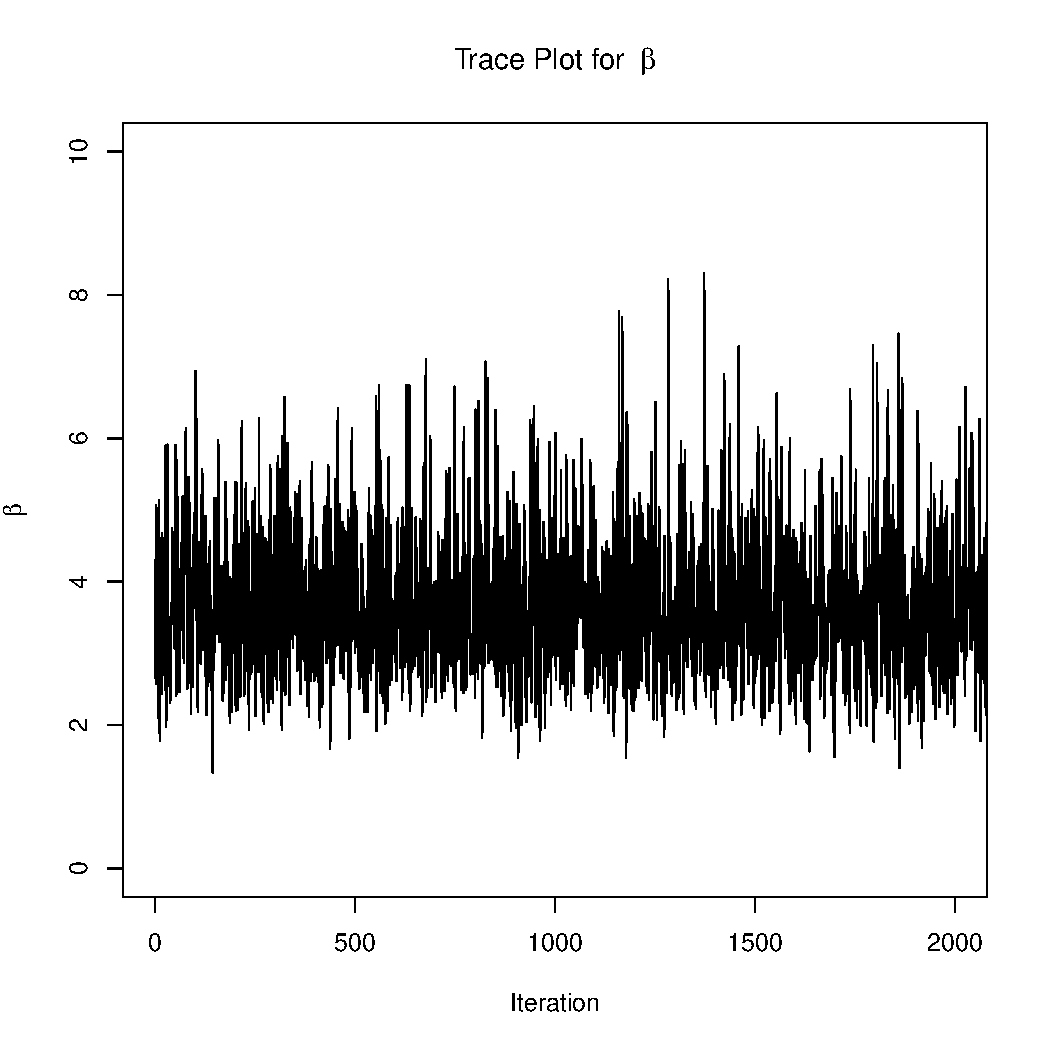
\includegraphics[scale=0.45]{betat100.pdf}
\label{betat100}}
\caption{Trace plot for $\alpha$ in Figure \ref{alphat100} and $\beta$ in Figure \ref{betat100} with a thin of 100}
\end{figure}

\begin{figure}
\centering
\subfloat[]
  {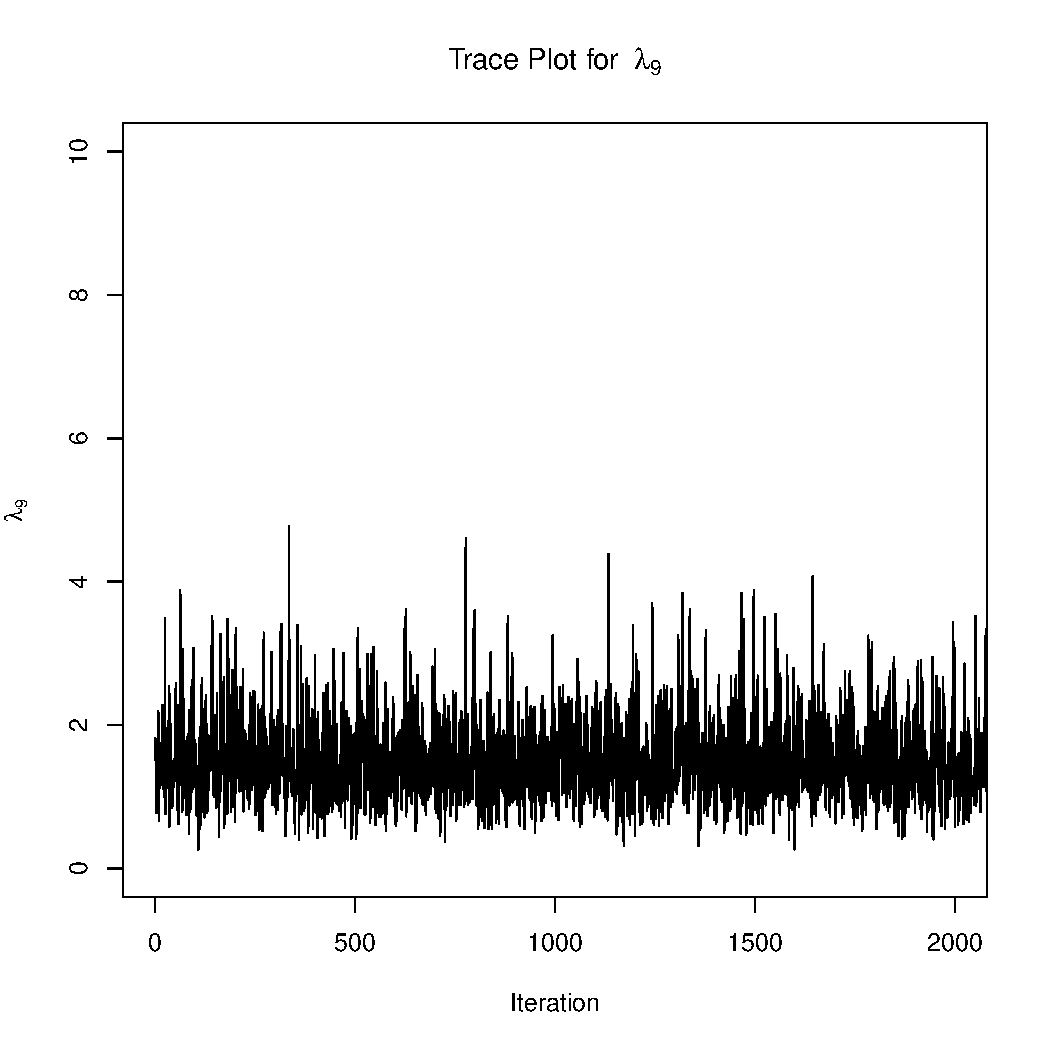
\includegraphics[scale=0.38]{tracelmd9t100.pdf}
\label{tracelmd9t100}}
\subfloat[]
  {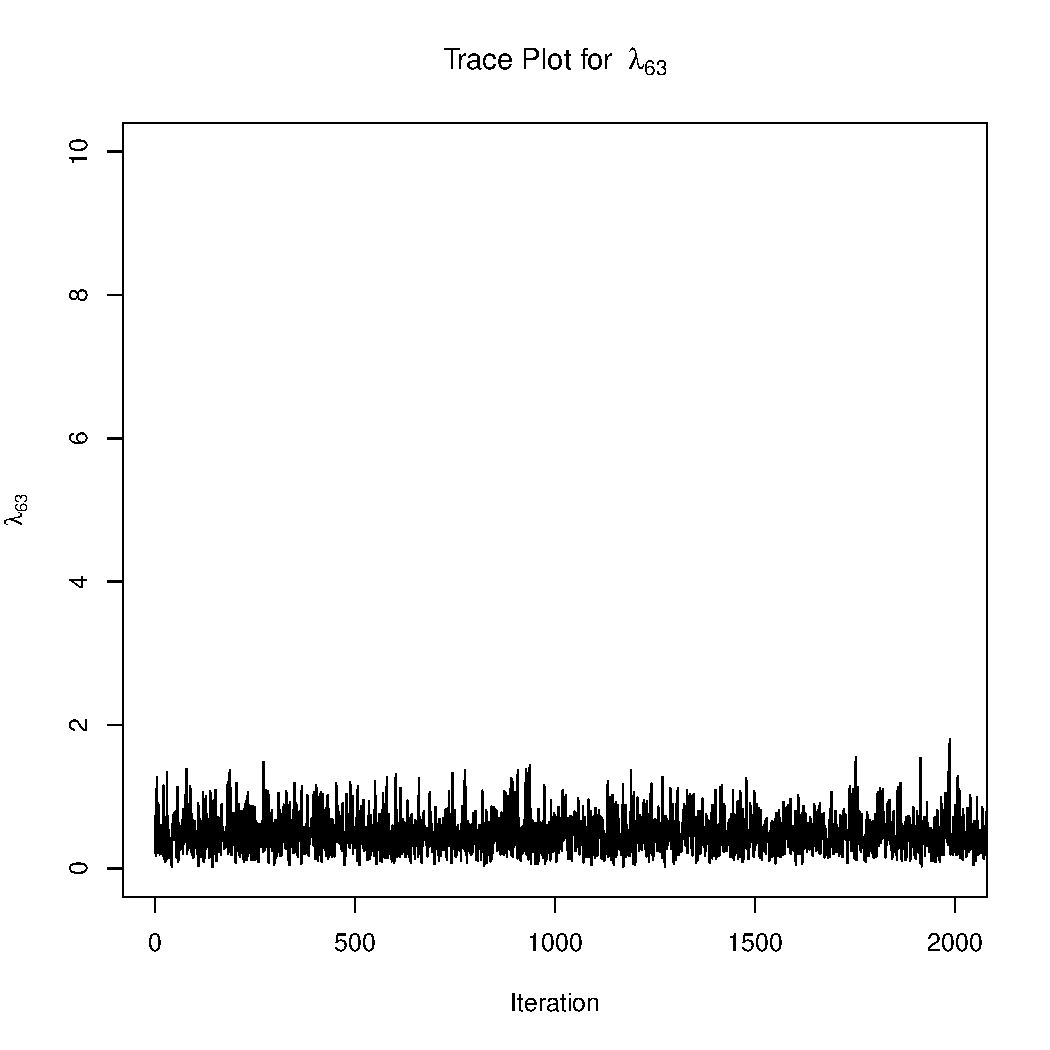
\includegraphics[scale=0.38]{tracelmd63t100.pdf}
\label{tracelmd63t100}}
\centering
\qquad
\centering
\subfloat[]
  {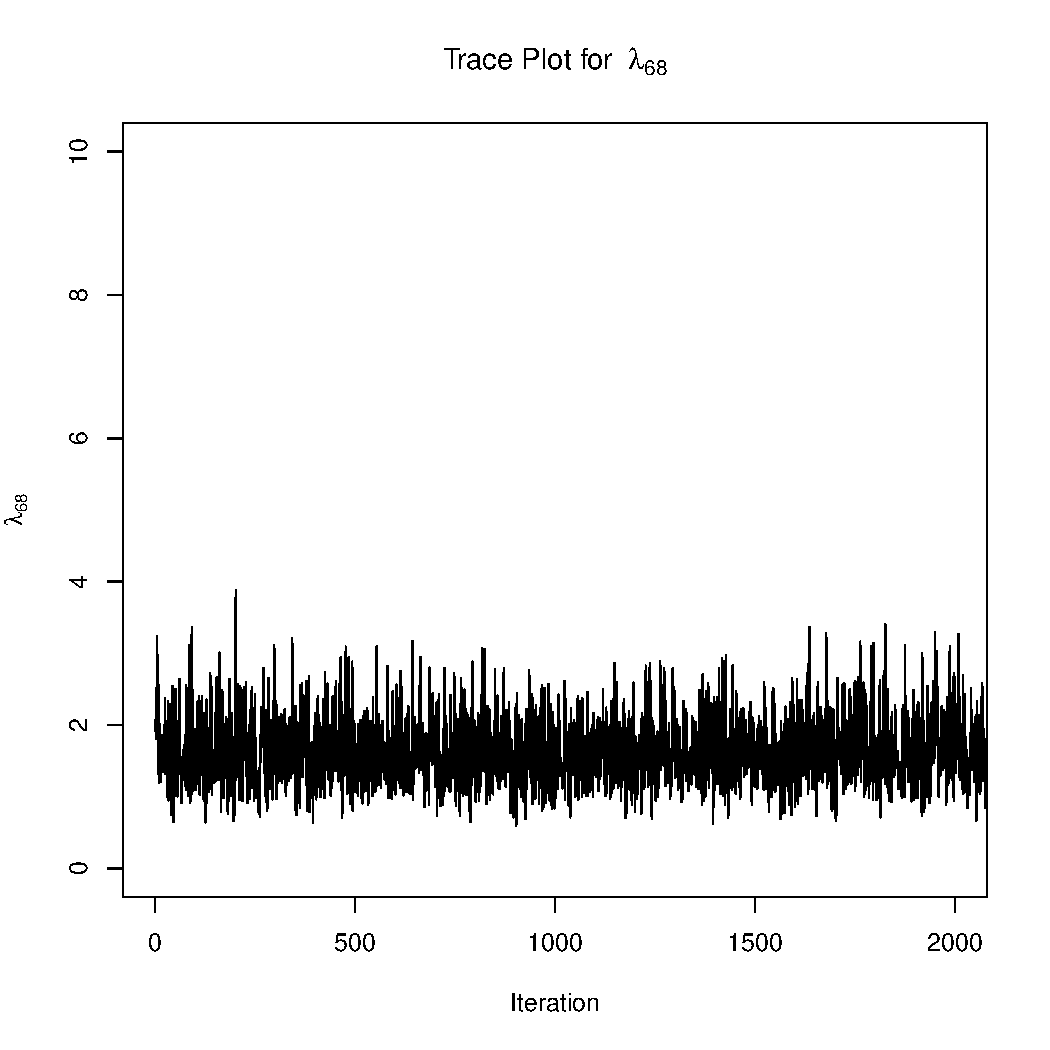
\includegraphics[scale=0.38]{tracelmd68t100.pdf}
\label{tracelmd68t100}}
\subfloat[]
  {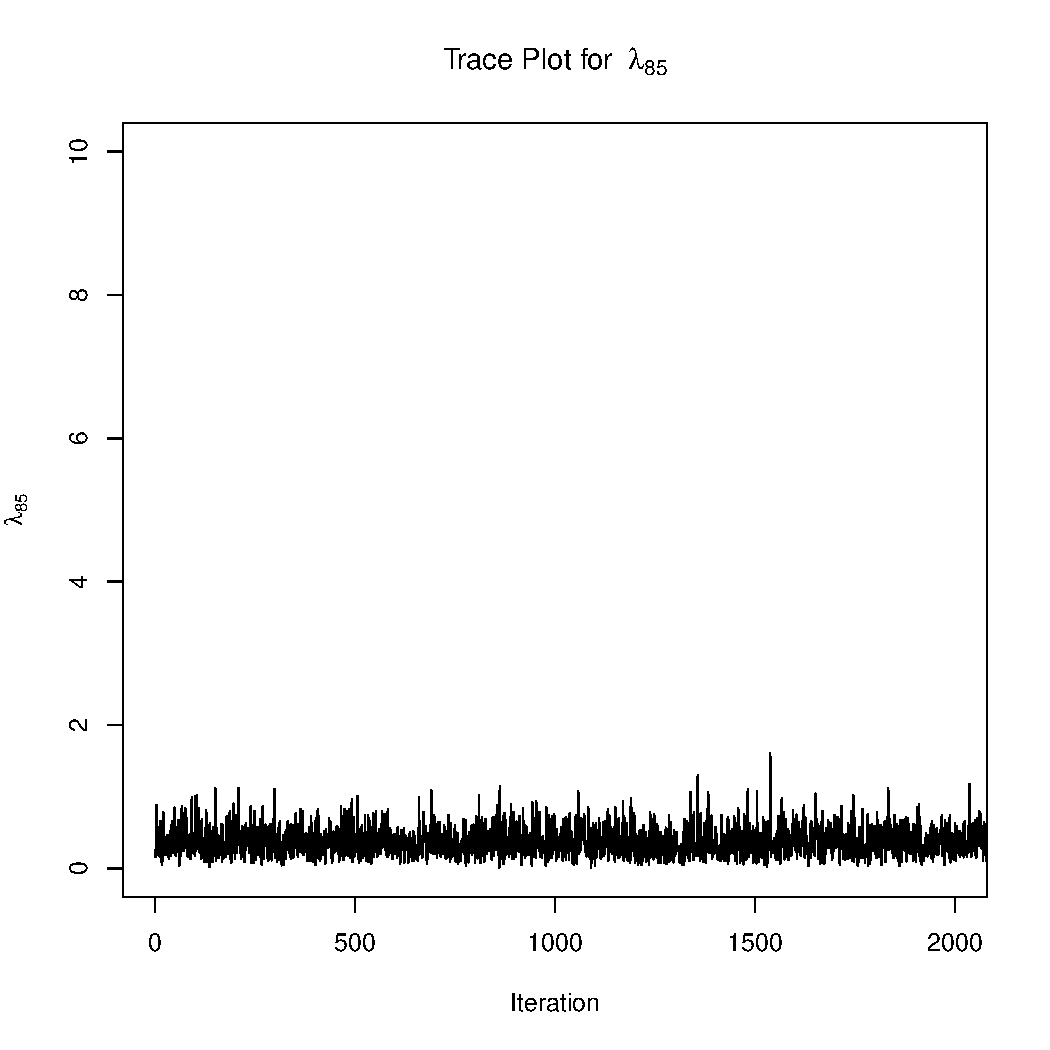
\includegraphics[scale=0.38]{tracelmd85t100.pdf}
\label{tracelmd85t100}}
\caption{Trace Plots for $\lambda_i$ using a thin of 100}
\label{tracet100}
\end{figure}

\begin{figure}
\centering
\subfloat[]
  {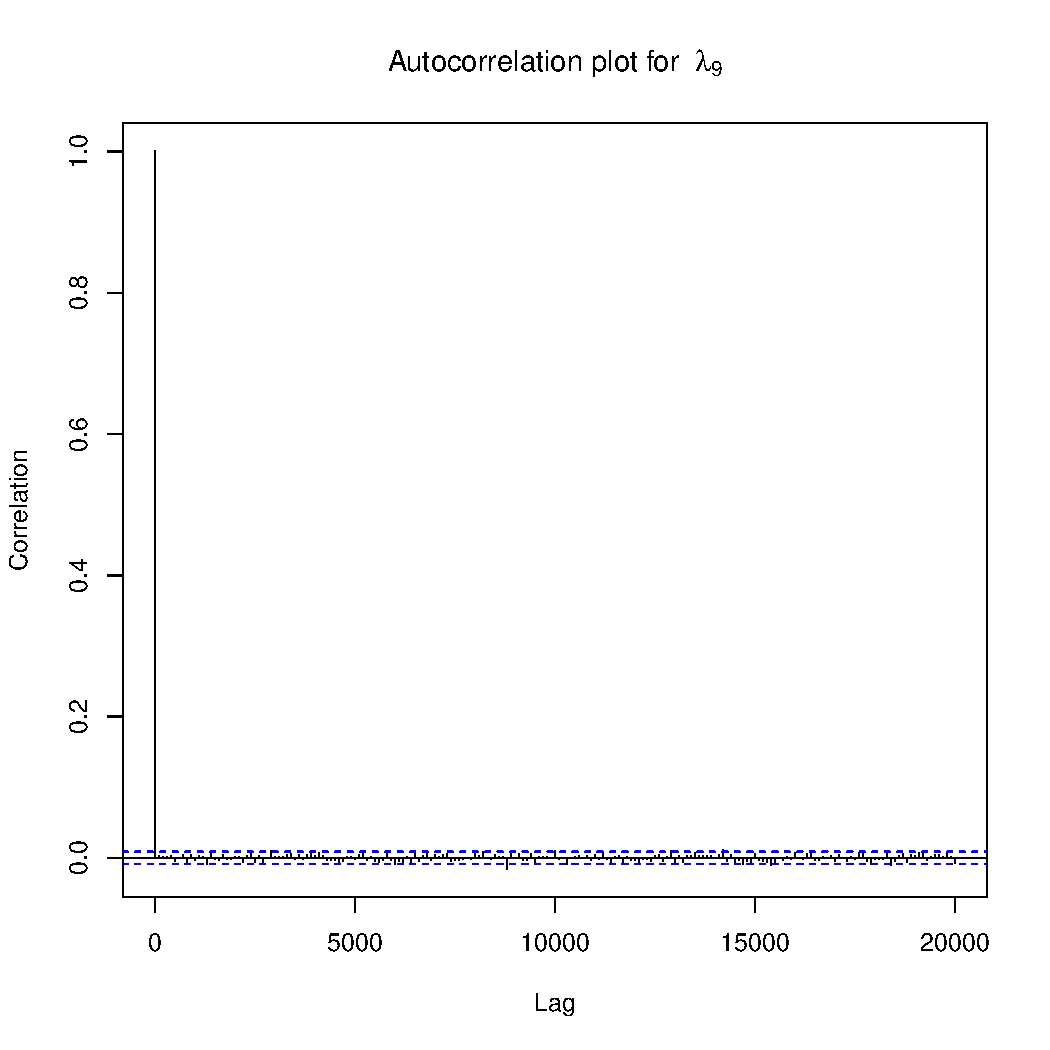
\includegraphics[scale=0.38]{acf9t100.pdf}
\label{acf9t100}}
\subfloat[]
  {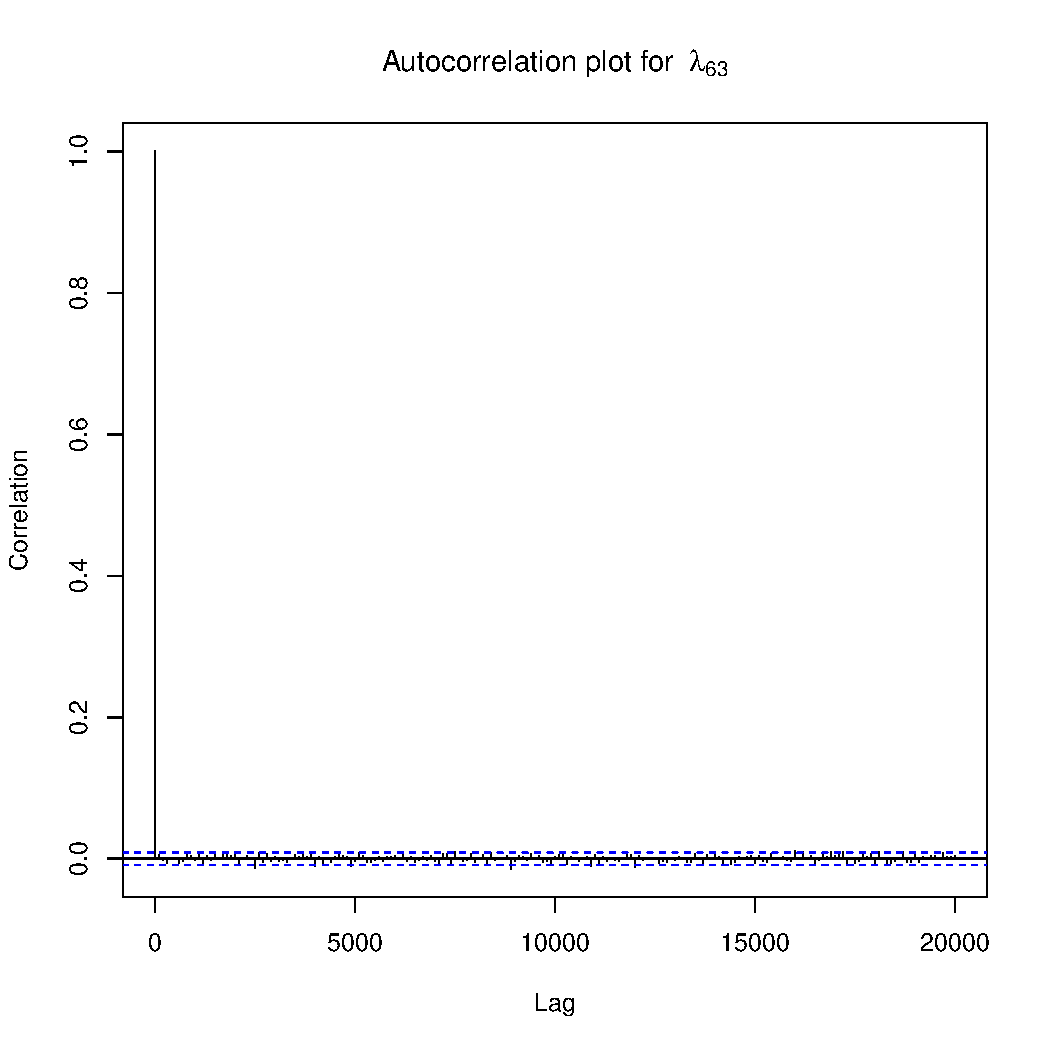
\includegraphics[scale=0.38]{acf63t100.pdf}
\label{acf63t100}}
\centering
\qquad
\centering
\subfloat[]
  {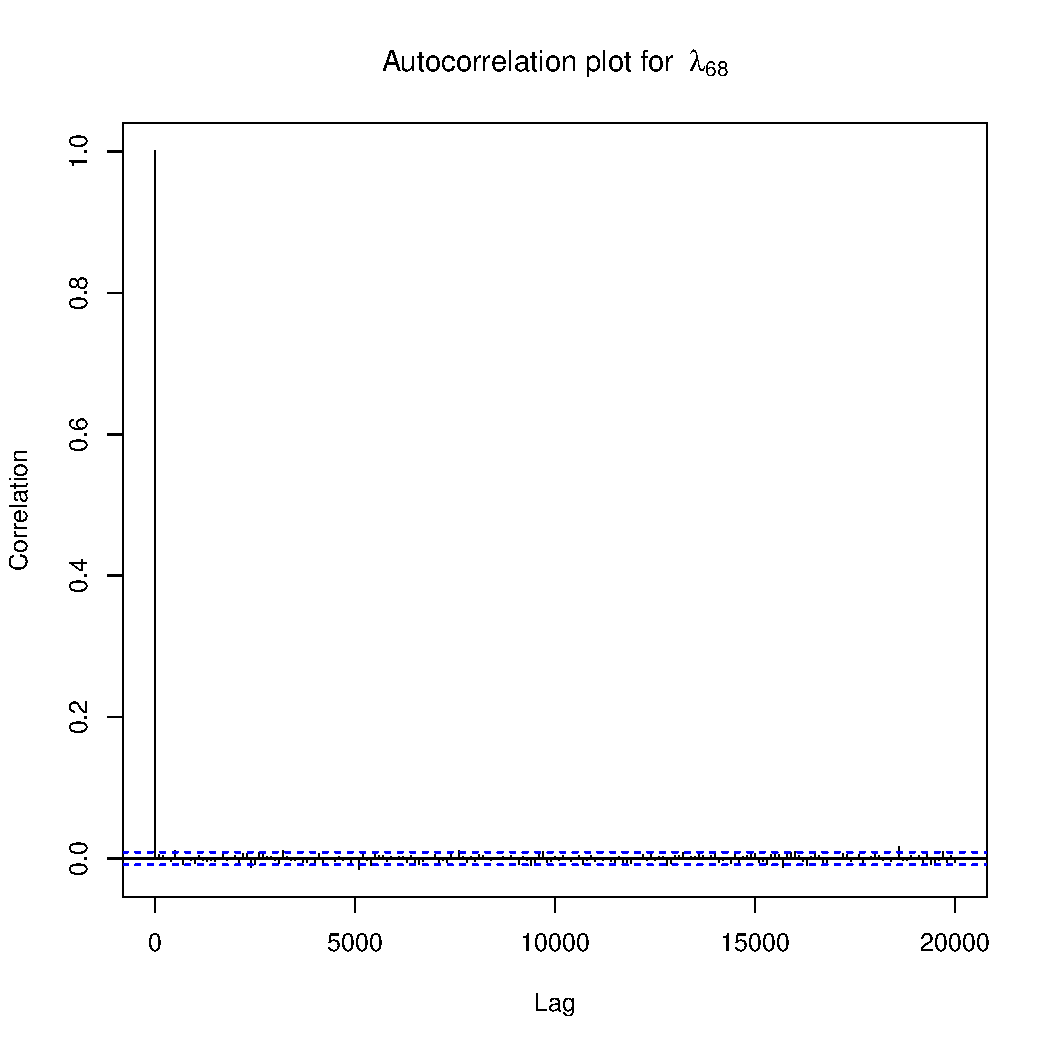
\includegraphics[scale=0.38]{acf68t100.pdf}
\label{acf68t100}}
\subfloat[]
  {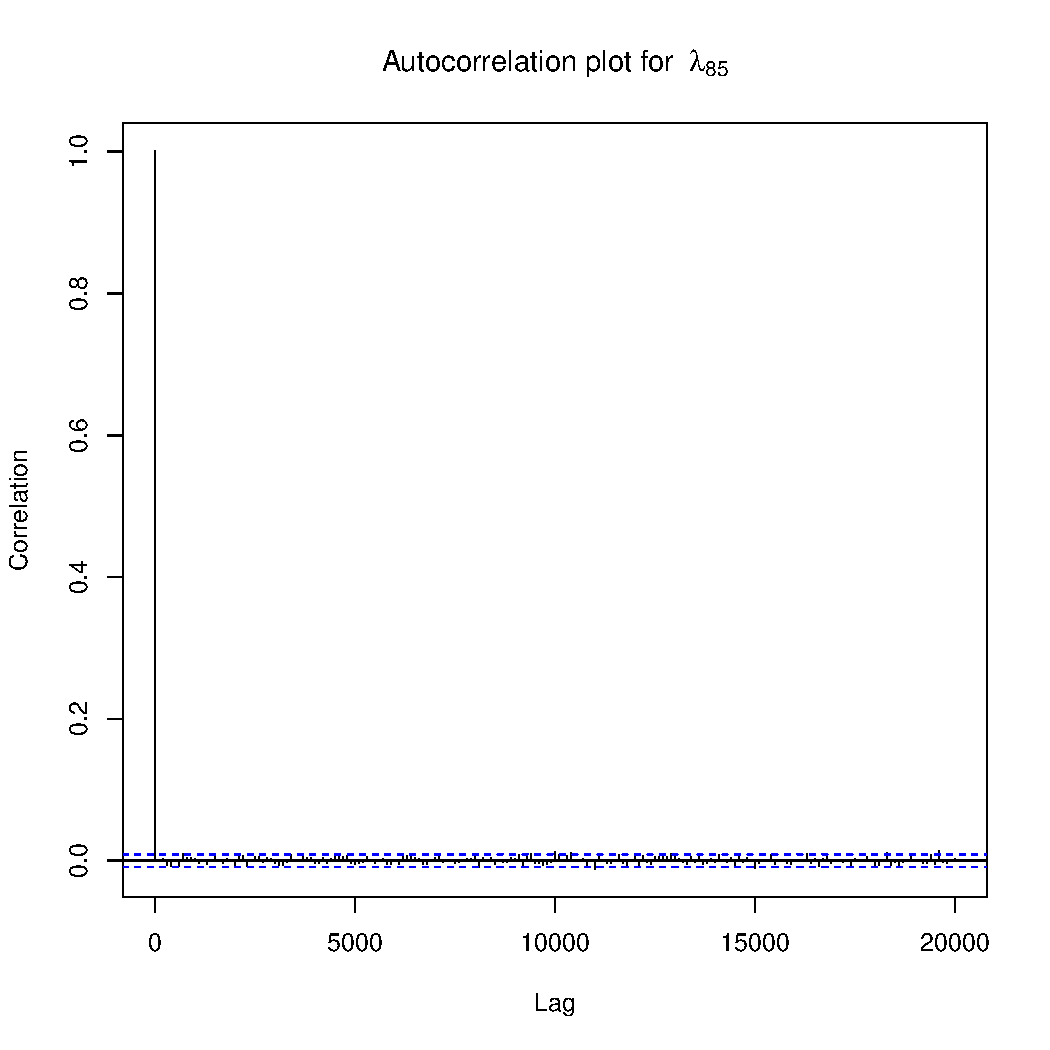
\includegraphics[scale=0.38]{acf85t100.pdf}
\label{acf85t100}}
\caption{Autocorrelation Plots for $\lambda_i$ using a thin of 100}
\label{acft100}
\end{figure}

%\end{landscape}

\begin{table}[ht]
\centering
\scalebox{0.7}{
\begin{tabular}{r|r|r|r|r|r|r|r|r|r}
  \hline
\hline
i & Mean & SE & SE(BM) & SE(TS) & i & Mean & SE & SE(BM) & SE(TS) \\ 
  \hline
1 & 0.843 & 0.0021 & 0.0023 & 0.0022 & 48 & 1.031 & 0.0018 & 0.0021 & 0.0019 \\ 
  2 & 0.829 & 0.0020 & 0.0023 & 0.0022 & 49 & 0.587 & 0.0015 & 0.0026 & 0.0024 \\ 
  3 & 1.304 & 0.0026 & 0.0041 & 0.0036 & 50 & 0.605 & 0.0015 & 0.0024 & 0.0023 \\ 
  4 & 1.047 & 0.0023 & 0.0028 & 0.0024 & 51 & 0.851 & 0.0017 & 0.0018 & 0.0017 \\ 
  5 & 1.000 & 0.0022 & 0.0022 & 0.0023 & 52 & 1.325 & 0.0021 & 0.0029 & 0.0026 \\ 
  6 & 0.717 & 0.0018 & 0.0023 & 0.0020 & 53 & 1.257 & 0.0020 & 0.0026 & 0.0024 \\ 
  7 & 0.762 & 0.0019 & 0.0025 & 0.0022 & 54 & 0.752 & 0.0016 & 0.0018 & 0.0017 \\ 
  8 & 0.899 & 0.0019 & 0.0020 & 0.0020 & 55 & 0.729 & 0.0016 & 0.0019 & 0.0019 \\ 
  9 & 1.511 & 0.0028 & 0.0048 & 0.0048 & 56 & 0.872 & 0.0015 & 0.0016 & 0.0015 \\ 
  10 & 0.751 & 0.0019 & 0.0024 & 0.0021 & 57 & 0.717 & 0.0015 & 0.0018 & 0.0017 \\ 
  11 & 0.801 & 0.0020 & 0.0022 & 0.0021 & 58 & 0.706 & 0.0015 & 0.0018 & 0.0018 \\ 
  12 & 0.832 & 0.0018 & 0.0018 & 0.0019 & 59 & 0.978 & 0.0017 & 0.0018 & 0.0018 \\ 
  13 & 0.785 & 0.0019 & 0.0024 & 0.0022 & 60 & 0.627 & 0.0014 & 0.0019 & 0.0018 \\ 
  14 & 1.176 & 0.0023 & 0.0030 & 0.0027 & 61 & 0.867 & 0.0017 & 0.0017 & 0.0017 \\ 
  15 & 1.381 & 0.0025 & 0.0039 & 0.0038 & 62 & 1.371 & 0.0021 & 0.0030 & 0.0026 \\ 
  16 & 0.726 & 0.0018 & 0.0022 & 0.0020 & 63 & 0.467 & 0.0012 & 0.0024 & 0.0024 \\ 
  17 & 0.704 & 0.0017 & 0.0023 & 0.0022 & 64 & 0.720 & 0.0014 & 0.0018 & 0.0015 \\ 
  18 & 1.218 & 0.0022 & 0.0030 & 0.0027 & 65 & 0.881 & 0.0017 & 0.0018 & 0.0018 \\ 
  19 & 0.623 & 0.0013 & 0.0019 & 0.0018 & 66 & 0.695 & 0.0015 & 0.0020 & 0.0018 \\ 
  20 & 0.939 & 0.0020 & 0.0020 & 0.0021 & 67 & 0.693 & 0.0013 & 0.0016 & 0.0015 \\ 
  21 & 0.935 & 0.0020 & 0.0020 & 0.0021 & 68 & 1.643 & 0.0022 & 0.0039 & 0.0037 \\ 
  22 & 0.933 & 0.0020 & 0.0020 & 0.0021 & 69 & 1.322 & 0.0020 & 0.0027 & 0.0024 \\ 
  23 & 1.481 & 0.0025 & 0.0046 & 0.0044 & 70 & 0.570 & 0.0012 & 0.0021 & 0.0019 \\ 
  24 & 1.276 & 0.0023 & 0.0034 & 0.0032 & 71 & 1.263 & 0.0019 & 0.0021 & 0.0021 \\ 
  25 & 1.195 & 0.0021 & 0.0028 & 0.0024 & 72 & 0.977 & 0.0016 & 0.0017 & 0.0016 \\ 
  26 & 0.813 & 0.0018 & 0.0019 & 0.0019 & 73 & 0.572 & 0.0012 & 0.0019 & 0.0018 \\ 
  27 & 0.716 & 0.0018 & 0.0024 & 0.0021 & 74 & 0.848 & 0.0015 & 0.0016 & 0.0015 \\ 
  28 & 1.110 & 0.0022 & 0.0025 & 0.0023 & 75 & 1.033 & 0.0016 & 0.0018 & 0.0016 \\ 
  29 & 1.052 & 0.0021 & 0.0023 & 0.0022 & 76 & 0.596 & 0.0012 & 0.0017 & 0.0016 \\ 
  30 & 1.438 & 0.0025 & 0.0042 & 0.0039 & 77 & 0.747 & 0.0012 & 0.0014 & 0.0013 \\ 
  31 & 1.392 & 0.0024 & 0.0038 & 0.0035 & 78 & 0.725 & 0.0013 & 0.0016 & 0.0014 \\ 
  32 & 1.287 & 0.0023 & 0.0033 & 0.0030 & 79 & 0.934 & 0.0015 & 0.0017 & 0.0016 \\ 
  33 & 1.063 & 0.0021 & 0.0022 & 0.0021 & 80 & 1.026 & 0.0016 & 0.0017 & 0.0016 \\ 
  34 & 1.285 & 0.0022 & 0.0029 & 0.0027 & 81 & 0.633 & 0.0012 & 0.0017 & 0.0014 \\ 
  35 & 0.878 & 0.0019 & 0.0021 & 0.0020 & 82 & 0.987 & 0.0014 & 0.0015 & 0.0015 \\ 
  36 & 1.220 & 0.0022 & 0.0029 & 0.0026 & 83 & 1.322 & 0.0018 & 0.0023 & 0.0020 \\ 
  37 & 0.705 & 0.0017 & 0.0022 & 0.0020 & 84 & 0.570 & 0.0009 & 0.0012 & 0.0011 \\ 
  38 & 1.475 & 0.0025 & 0.0044 & 0.0039 & 85 & 0.367 & 0.0009 & 0.0022 & 0.0021 \\ 
  39 & 0.851 & 0.0018 & 0.0019 & 0.0019 & 86 & 0.982 & 0.0014 & 0.0015 & 0.0015 \\ 
  40 & 1.049 & 0.0021 & 0.0023 & 0.0021 & 87 & 1.253 & 0.0017 & 0.0021 & 0.0019 \\ 
  41 & 1.216 & 0.0022 & 0.0028 & 0.0026 & 88 & 1.080 & 0.0015 & 0.0016 & 0.0015 \\ 
  42 & 1.353 & 0.0023 & 0.0033 & 0.0032 & 89 & 0.657 & 0.0012 & 0.0015 & 0.0013 \\ 
  43 & 1.409 & 0.0024 & 0.0039 & 0.0036 & 90 & 0.609 & 0.0011 & 0.0015 & 0.0013 \\ 
  44 & 0.901 & 0.0018 & 0.0018 & 0.0018 & 91 & 1.092 & 0.0014 & 0.0016 & 0.0014 \\ 
  45 & 1.031 & 0.0020 & 0.0022 & 0.0021 & 92 & 0.795 & 0.0011 & 0.0012 & 0.0011 \\ 
  46 & 1.243 & 0.0021 & 0.0027 & 0.0024 & 93 & 1.374 & 0.0013 & 0.0016 & 0.0014 \\ 
  47 & 0.919 & 0.0018 & 0.0019 & 0.0019 & 94 & 1.300 & 0.0013 & 0.0016 & 0.0014 \\ 
   \hline
   \hline
\end{tabular}
}

\caption{Estimated Mortality Rates ($\bar{\lambda}_i$) for Hospitals 1
  to 94 using a thin of 1} 
\label{mean1}
\end{table}

\begin{table}[ht]
\centering
\scalebox{0.7}{
\begin{tabular}{r|r|r|r|r|r|r|r|r|r}
  \hline
\hline
i & Mean & SE & SE(BM) & SE(TS) & i & Mean & SE & SE(BM) & SE(TS) \\ 
  \hline
  \hline
1 & 0.844 & 0.0021 & 0.0022 & 0.0021 & 48 & 1.034 & 0.0019 & 0.0020 & 0.0019 \\ 
  2 & 0.832 & 0.0021 & 0.0022 & 0.0021 & 49 & 0.587 & 0.0014 & 0.0014 & 0.0014 \\ 
  3 & 1.300 & 0.0026 & 0.0026 & 0.0026 & 50 & 0.603 & 0.0015 & 0.0013 & 0.0015 \\ 
  4 & 1.046 & 0.0023 & 0.0021 & 0.0023 & 51 & 0.850 & 0.0017 & 0.0015 & 0.0016 \\ 
  5 & 1.002 & 0.0022 & 0.0021 & 0.0022 & 52 & 1.323 & 0.0021 & 0.0021 & 0.0021 \\ 
  6 & 0.716 & 0.0018 & 0.0018 & 0.0018 & 53 & 1.264 & 0.0020 & 0.0021 & 0.0020 \\ 
  7 & 0.760 & 0.0019 & 0.0017 & 0.0019 & 54 & 0.750 & 0.0016 & 0.0016 & 0.0016 \\ 
  8 & 0.895 & 0.0019 & 0.0019 & 0.0019 & 55 & 0.725 & 0.0016 & 0.0017 & 0.0016 \\ 
  9 & 1.512 & 0.0028 & 0.0028 & 0.0028 & 56 & 0.870 & 0.0016 & 0.0016 & 0.0016 \\ 
  10 & 0.751 & 0.0019 & 0.0017 & 0.0019 & 57 & 0.719 & 0.0015 & 0.0015 & 0.0015 \\ 
  11 & 0.804 & 0.0020 & 0.0019 & 0.0020 & 58 & 0.708 & 0.0015 & 0.0016 & 0.0015 \\ 
  12 & 0.834 & 0.0018 & 0.0018 & 0.0018 & 59 & 0.976 & 0.0017 & 0.0017 & 0.0017 \\ 
  13 & 0.784 & 0.0019 & 0.0020 & 0.0019 & 60 & 0.628 & 0.0014 & 0.0013 & 0.0013 \\ 
  14 & 1.175 & 0.0023 & 0.0022 & 0.0024 & 61 & 0.865 & 0.0017 & 0.0018 & 0.0017 \\ 
  15 & 1.383 & 0.0025 & 0.0026 & 0.0025 & 62 & 1.373 & 0.0021 & 0.0020 & 0.0021 \\ 
  16 & 0.730 & 0.0018 & 0.0018 & 0.0018 & 63 & 0.468 & 0.0012 & 0.0012 & 0.0012 \\ 
  17 & 0.706 & 0.0017 & 0.0019 & 0.0017 & 64 & 0.720 & 0.0014 & 0.0015 & 0.0014 \\ 
  18 & 1.221 & 0.0022 & 0.0023 & 0.0022 & 65 & 0.883 & 0.0017 & 0.0016 & 0.0017 \\ 
  19 & 0.623 & 0.0013 & 0.0013 & 0.0013 & 66 & 0.693 & 0.0015 & 0.0014 & 0.0015 \\ 
  20 & 0.939 & 0.0020 & 0.0020 & 0.0020 & 67 & 0.695 & 0.0013 & 0.0014 & 0.0013 \\ 
  21 & 0.934 & 0.0020 & 0.0020 & 0.0020 & 68 & 1.642 & 0.0022 & 0.0022 & 0.0022 \\ 
  22 & 0.934 & 0.0020 & 0.0020 & 0.0020 & 69 & 1.321 & 0.0020 & 0.0019 & 0.0020 \\ 
  23 & 1.481 & 0.0025 & 0.0026 & 0.0025 & 70 & 0.570 & 0.0012 & 0.0013 & 0.0012 \\ 
  24 & 1.274 & 0.0023 & 0.0024 & 0.0023 & 71 & 1.267 & 0.0019 & 0.0021 & 0.0019 \\ 
  25 & 1.198 & 0.0022 & 0.0020 & 0.0022 & 72 & 0.977 & 0.0016 & 0.0017 & 0.0016 \\ 
  26 & 0.817 & 0.0018 & 0.0018 & 0.0018 & 73 & 0.571 & 0.0012 & 0.0012 & 0.0012 \\ 
  27 & 0.716 & 0.0018 & 0.0018 & 0.0018 & 74 & 0.854 & 0.0015 & 0.0015 & 0.0015 \\ 
  28 & 1.110 & 0.0022 & 0.0022 & 0.0022 & 75 & 1.033 & 0.0016 & 0.0016 & 0.0016 \\ 
  29 & 1.053 & 0.0021 & 0.0022 & 0.0021 & 76 & 0.595 & 0.0012 & 0.0012 & 0.0012 \\ 
  30 & 1.439 & 0.0024 & 0.0023 & 0.0024 & 77 & 0.747 & 0.0012 & 0.0012 & 0.0012 \\ 
  31 & 1.390 & 0.0024 & 0.0022 & 0.0024 & 78 & 0.724 & 0.0013 & 0.0012 & 0.0013 \\ 
  32 & 1.288 & 0.0023 & 0.0024 & 0.0023 & 79 & 0.931 & 0.0015 & 0.0016 & 0.0015 \\ 
  33 & 1.062 & 0.0021 & 0.0021 & 0.0021 & 80 & 1.024 & 0.0016 & 0.0016 & 0.0016 \\ 
  34 & 1.283 & 0.0022 & 0.0023 & 0.0021 & 81 & 0.633 & 0.0012 & 0.0012 & 0.0012 \\ 
  35 & 0.878 & 0.0019 & 0.0019 & 0.0019 & 82 & 0.984 & 0.0014 & 0.0014 & 0.0014 \\ 
  36 & 1.219 & 0.0022 & 0.0022 & 0.0022 & 83 & 1.319 & 0.0018 & 0.0018 & 0.0018 \\ 
  37 & 0.705 & 0.0017 & 0.0017 & 0.0017 & 84 & 0.571 & 0.0009 & 0.0009 & 0.0009 \\ 
  38 & 1.476 & 0.0025 & 0.0025 & 0.0025 & 85 & 0.368 & 0.0009 & 0.0010 & 0.0009 \\ 
  39 & 0.852 & 0.0018 & 0.0018 & 0.0018 & 86 & 0.985 & 0.0014 & 0.0013 & 0.0014 \\ 
  40 & 1.049 & 0.0020 & 0.0021 & 0.0020 & 87 & 1.254 & 0.0017 & 0.0017 & 0.0017 \\ 
  41 & 1.216 & 0.0022 & 0.0021 & 0.0022 & 88 & 1.082 & 0.0015 & 0.0015 & 0.0015 \\ 
  42 & 1.352 & 0.0023 & 0.0023 & 0.0023 & 89 & 0.657 & 0.0012 & 0.0011 & 0.0011 \\ 
  43 & 1.407 & 0.0024 & 0.0025 & 0.0024 & 90 & 0.611 & 0.0011 & 0.0011 & 0.0011 \\ 
  44 & 0.906 & 0.0017 & 0.0018 & 0.0017 & 91 & 1.092 & 0.0014 & 0.0013 & 0.0014 \\ 
  45 & 1.030 & 0.0020 & 0.0020 & 0.0020 & 92 & 0.798 & 0.0011 & 0.0012 & 0.0011 \\ 
  46 & 1.246 & 0.0021 & 0.0020 & 0.0021 & 93 & 1.373 & 0.0013 & 0.0013 & 0.0013 \\ 
  47 & 0.918 & 0.0018 & 0.0018 & 0.0018 & 94 & 1.304 & 0.0013 & 0.0013 & 0.0013 \\ 
   \hline
   \hline
\end{tabular}
}
\caption{Estimated Mortality Rates ($\bar{\lambda}_i$) for Hospitals 1
  to 94 using a thin of 100} 
\label{mean100}
\end{table}

\clearpage

\paragraph{Appendix 1: model.txt}
\begin{verbatim}
model {
for (i in 1:N) {
Z[i] ~ dpois(lambda[i]*e[i])
lambda[i] ~ dgamma(alpha,beta)
}
z0 <- 0.53
a0 <- log(2)/z0
alpha ~ dexp(a0)
b0 <- 1
b1 <- 0.65
beta ~ dgamma(b0,b1)
}
\end{verbatim}

\paragraph{Appendix 2: script.txt}
\begin{verbatim}
model clear
data clear
model in "model.txt"
data in "data.txt"
compile
inits in "initial_1.txt"
initialize
update 10000
monitor beta, thin(100)
monitor alpha, thin(100)
monitor lambda, thin(100)
monitor Z, thin(100)
update 5000000
coda *
\end{verbatim}

\paragraph{Appendix 3: R code}
\begin{verbatim}
library(coda)
library(xtable)
data = read.table("ht-data.txt",header=TRUE)
attach(data)
length(e)
res = read.coda("CODAchain1.txt", "CODAindex.txt")

z0 = 0.53
a0 = log(2)/z0
b0 = 1
b1 = 0.65
logpost = matrix(0,dim(res)[1],1)
for(i in 1:94){
    temp1 <- log(dpois(round(res[,96+i]),res[,2+i]*e[i]))
    temp2 <- log(dgamma(res[,2+i],res[,2],rate = res[,1]))
    temp3 <- log(dexp(res[,2],rate=a0))
    temp4 <- log(dgamma(res[,1],b0,rate = b1))
    logpost = logpost + temp1 + temp2 + temp3 + temp4
}


colnames(res)

pdf("alpha.pdf")
plot(as.numeric(res[,2]),  type= 'l',xlim = c(0,2000),
     ylim = c(0,10),
xlab = "Iteration", ylab = expression(alpha),
     main = expression("Trace Plot for " ~ alpha))
##trace plot
dev.off()


pdf("beta.pdf")
plot(as.numeric(res[,1]),  type= 'l',xlim = c(0,2000),
     ylim = c(0,10),
xlab = "Iteration", ylab = expression(beta),
     main = expression("Trace Plot for " ~ beta))
##trace plot
dev.off()

pdf("tracelmd9.pdf")
plot(as.numeric(res[,2+9]),  type= 'l',xlim = c(0,2000),
     ylim = c(0,10),
xlab = "Iteration", ylab = expression(lambda[9]),
     main=expression("Trace Plot for " ~ lambda[9]))
##trace plot
dev.off()
pdf("acf9.pdf")
acf(res[,2+9], lag.max = 200, xlab = "Lag",
    ylab = "Correlation",
    main=expression("Autocorrelation plot for " ~ lambda[9]))
## autocorrelation plot
dev.off()

pdf("tracelmd63.pdf")
plot(as.numeric(res[,2+63]),  type= 'l',xlim = c(0,2000),
     ylim = c(0,10),
xlab = "Iteration", ylab = expression(lambda[63]),
     main=expression("Trace Plot for " ~ lambda[63]))
##trace plot
dev.off()
pdf("acf63.pdf")
acf(res[,2+63], lag.max = 200, xlab = "Lag",
    ylab = "Correlation",
    main=expression("Autocorrelation plot for " ~ lambda[63]))
## autocorrelation plot
dev.off()

pdf("tracelmd68.pdf")
plot(as.numeric(res[,2+68]),  type= 'l',xlim = c(0,2000),
     ylim = c(0,10),
xlab = "Iteration", ylab = expression(lambda[68]),
     main=expression("Trace Plot for " ~ lambda[68]))
##trace plot
dev.off()
pdf("acf68.pdf")
acf(res[,2+68], lag.max = 200, xlab = "Lag",
    ylab = "Correlation",
    main=expression("Autocorrelation plot for " ~ lambda[68]))
## autocorrelation plot
dev.off()

pdf("tracelmd85.pdf")
plot(as.numeric(res[,2+85]),  type= 'l',xlim = c(0,2000),
     ylim = c(0,10),
xlab = "Iteration", ylab = expression(lambda[85]),
     main=expression("Trace Plot for " ~ lambda[85]))
##trace plot
dev.off()
pdf("acf85.pdf")
acf(res[,2+85], lag.max = 200, xlab = "Lag",
    ylab = "Correlation",
    main=expression("Autocorrelation plot for " ~ lambda[85]))
## autocorrelation plot
dev.off()

pdf("logpost.pdf")
plot(as.numeric(-logpost),  type= 'l',xlim = c(0,2000),
xlab = "Iteration", ylab = "Negative Log Posterior" ,
     main = "Negative Log Posterior" )
##plot for log posterior
dev.off()

pdf("cumsum.pdf")
x = cumsum(-logpost)/1:dim(res)[1]
plot(x,  type= 'l',
     ylab = "Cumulative Average of Negative Log Posterior",
     main = "Cumulative Average of Negative Log Posterior")
dev.off()

jpeg("cumsum.jpeg")
x = cumsum(-logpost)/1:dim(res)[1]
plot(x,  type= 'l',
     ylab = "Cumulative Average of Negative Log Posterior")
dev.off()

pdf("acf.pdf")
acf(res[,3], lag.max = 200, xlab = "Lag", ylab = "Correlation",
    main="")
## autocorrelation plot
dev.off()

pdf("alphaacf.pdf")
acf(res[,2], lag.max = 200, xlab = "Lag", ylab = "Correlation",
    main=expression("Autocorrelation Plot for " ~ alpha))
## autocorrelation plot
dev.off()

pdf("betaacf.pdf")
acf(res[,1], lag.max = 200, xlab = "Lag", ylab = "Correlation",
    main=expression("Autocorrelation Plot for " ~ beta))
## autocorrelation plot
dev.off()

btchsz = floor(dim(res)[1]/sqrt(dim(res)[1]))
nbtch = floor(dim(res)[1]/btchsz)


meanlambda = matrix(0,94,1)
varlambda = matrix(0,94,1)

for(i in 1:94){
meanlambda[i] = mean(res[,2+i])

btchvar = matrix(0,nbtch,1)
for (j in 1:nbtch){
    lb = (j-1)*btchsz
    ub = j*btchsz
btchvar[j] = var(res[lb:ub,2+i])
}

varlambda[i] = (btchsz/(nbtch-1))*sum((btchvar - var(res[,2+i]))^2) 

}

res.sum = summary(res[,1:96])
d.res.sum = as.data.frame(res.sum$statistics)
dim(d.res.sum)

bS=floor(dim(res)[1]/sqrt(dim(res)[1]))

library(xtable)
temp = as.data.frame(cbind(1:47, meanlambda[1:47],
    d.res.sum[(1+2):(47+2),3],
    as.matrix(batchSE(res[,1:96],batchSize=bS)[(1+2):(47+2)]),
    d.res.sum[(1+2):(47+2),4], 48:94, meanlambda[48:94],
    d.res.sum[(48+2):(94+2),3],
    as.matrix(batchSE(res[,1:96],
                      batchSize=bS)[(48+2):(94+2)]),
    d.res.sum[(48+2):(94+2),4]))
colnames(temp) =
    c("i","Mean","SE","SE(BM)","SE(TS)","i",
      "Mean","SE","SE(BM)","SE(TS)")
temptab = xtable(temp,
    caption="Estimated means for $\\lambda_i$",
    label="tab1",digits=c(0,0,3,4,4,4,0,3,4,4,4))
print(temptab,include.rownames=FALSE)
\end{verbatim}

 
\end{document}